\documentclass[a4paper]{article}

% CJK support: prefer ctex, fallback to XeTeX native line breaking
\IfFileExists{ctex.sty}{
  \usepackage[fontset=fandol]{ctex}
}{
  % Fallback for minimal TeX installs (e.g. MacTeX Basic, TeX Live scheme-basic)
  % without ctex/xeCJK. Uses XeTeX's built-in CJK line breaking.
  \usepackage{fontspec}
  \XeTeXlinebreaklocale "zh"
  \XeTeXlinebreakskip = 0pt plus 1pt
  \IfFontExistsTF{Songti SC}{\setmainfont{Songti SC}}{%
    \IfFontExistsTF{Noto Serif CJK SC}{\setmainfont{Noto Serif CJK SC}}{}%
  }
  \IfFontExistsTF{Heiti SC}{\setsansfont{Heiti SC}}{%
    \IfFontExistsTF{Noto Sans CJK SC}{\setsansfont{Noto Sans CJK SC}}{}%
  }
}

% Basic packages
\usepackage{amsmath, amssymb}
\usepackage{graphicx}
\usepackage[margin=2.5cm]{geometry}
\emergencystretch=3em
\usepackage[most]{tcolorbox}
\usepackage{etoolbox}
\usepackage{listings}
\usepackage{hyperref}
\usepackage{booktabs}
\usepackage{array}
\usepackage{subcaption}
\usepackage{float}
\usepackage{tikz}
\IfFileExists{pgfplots.sty}{
    \usepackage{pgfplots}
    \pgfplotsset{compat=1.18}
}{}

% ===== Highlight boxes =====
\newtcolorbox{knowledgebox}[1]{
    enhanced, colback=blue!5!white, colframe=blue!75!black, colbacktitle=blue!75!black,
    coltitle=white, fonttitle=\bfseries, title={#1}, attach boxed title to top left={yshift=-2mm, xshift=2mm},
    boxrule=1pt, sharp corners
}

\newtcolorbox{importantbox}[1]{
    enhanced, colback=yellow!10!white, colframe=yellow!80!black, colbacktitle=yellow!80!black,
    coltitle=black, fonttitle=\bfseries, title={#1}, sharp corners
}

\newtcolorbox{warningbox}[1]{
    enhanced, colback=red!5!white, colframe=red!75!black, colbacktitle=red!75!black,
    coltitle=white, fonttitle=\bfseries, title={#1}, sharp corners
}

\newtcolorbox{practicebox}[1]{
    enhanced, colback=black!3!white, colframe=black!75, colbacktitle=black!75,
    coltitle=white, fonttitle=\bfseries, title={#1}, sharp corners
}

% ===== Code listings =====
\lstset{
    basicstyle=\ttfamily\small,
    keywordstyle=\color{blue},
    stringstyle=\color{red!60!black},
    commentstyle=\color{green!60!black},
    breaklines=true,
    frame=single,
    numbers=left,
    numberstyle=\tiny\color{gray},
    captionpos=b,
    extendedchars=false
}

% ===== Figure provenance and unit macros =====
% \vtag goes inside \caption{...}; \srcnote{MM:SS--MM:SS} follows the figure environment.
\newcommand{\vtag}{\protect\footnotemark}
\newcommand{\srcnote}[1]{\footnotetext{视频画面时间区间：#1。若为裁剪图，时间区间仍对应原视频画面。}}
% Units work in text and math mode; never hand-write $^\circ$ or \AA inside \mathrm.
\newcommand{\degC}{\ensuremath{^{\circ}\mathrm{C}}}
\newcommand{\um}{\ensuremath{\mu\mathrm{m}}}
\newcommand{\nm}{\ensuremath{\mathrm{nm}}}
\newcommand{\angstrom}{\ensuremath{\text{\AA}}}

% ===== Front-page metadata =====
% Fill these in when generating notes.
\newcommand{\notetitle}{深度学习中的数学}
\newcommand{\notesubtitle}{GAMES001 图形学中的数学 · 第 14 集：生成模型的案例分析：VAE 与扩散模型}
\newcommand{\noteauthors}{根据 GAMES-Webinar 直播录像整理（阮良旺 主讲）}
\newcommand{\notedate}{2024年7月1日（直播）}
\newcommand{\videochannel}{GAMES-Webinar（哔哩哔哩）}
\newcommand{\videopublishdate}{2024年3月6日（合集）}
\newcommand{\videoduration}{1小时20分0秒}
\newcommand{\videourl}{https://www.bilibili.com/video/BV1MF4m1V7e3/?p=14}
\newcommand{\videocoverpath}{cover.jpg}

\begin{document}

% ===== Title page =====
\begin{titlepage}
\centering
{\Large 课程笔记\par}
\vspace{1.2cm}
{\huge\bfseries \notetitle\par}
\ifdefempty{\notesubtitle}{}{
\vspace{0.3cm}
{\large \notesubtitle\par}
}
\vspace{0.5cm}
{\large \noteauthors\par}
\vspace{0.3cm}
{\large \notedate\par}
\vspace{1.0cm}

\ifdefempty{\videocoverpath}{
{\small 请在生成笔记时填入视频封面图的本地路径。\par}
}{
\includegraphics[width=0.82\textwidth,height=0.40\textheight,keepaspectratio]{\videocoverpath}\par
}

\vfill
\begin{tcolorbox}[width=0.9\textwidth, colback=black!2!white, colframe=black!60, sharp corners]
\textbf{视频作者/频道}：\videochannel\par
\textbf{发布日期}：\videopublishdate\par
\textbf{视频时长}：\videoduration\par
\textbf{视频链接}：
\ifdefempty{\videourl}{
未填写
}{
\href{\videourl}{\nolinkurl{\videourl}}
}
\end{tcolorbox}
\end{titlepage}

\tableofcontents
\newpage

%% --- 正文内容开始 --- %%

\section{这一讲讲什么}

第十四集对应课程的第十五讲，由阮良旺主讲，主题是深度学习中的数学，以生成模型作为案例分析。讲者说，之前的课程介绍了概率论、线性代数等很多基础性的内容；随着图形学和深度学习技术的发展，后来的很多工作都与深度学习相关，而深度学习领域本身也在不断发展。

深度学习中用到的数学方方面面都有，网上有一些非常好的教程，包括微积分、线性代数、概率论、优化等。讲者说今天的想法不是把它们全部讲一遍，而是从几个具体案例的角度，看看概率论这些基础数学如何和前沿的工作建立联系。他也坦言，从“一加一等于二”这样的基础，到 Transformer、NeRF、扩散模型这样的前沿成果，中间有比较大的差距，一节课不可能把它填上。所以理解推导的关键部分在课件上用红色标出，其他细节可以课后自己推一推。

\noindent\begin{minipage}{\textwidth}
\begin{figure}[H]
\centering
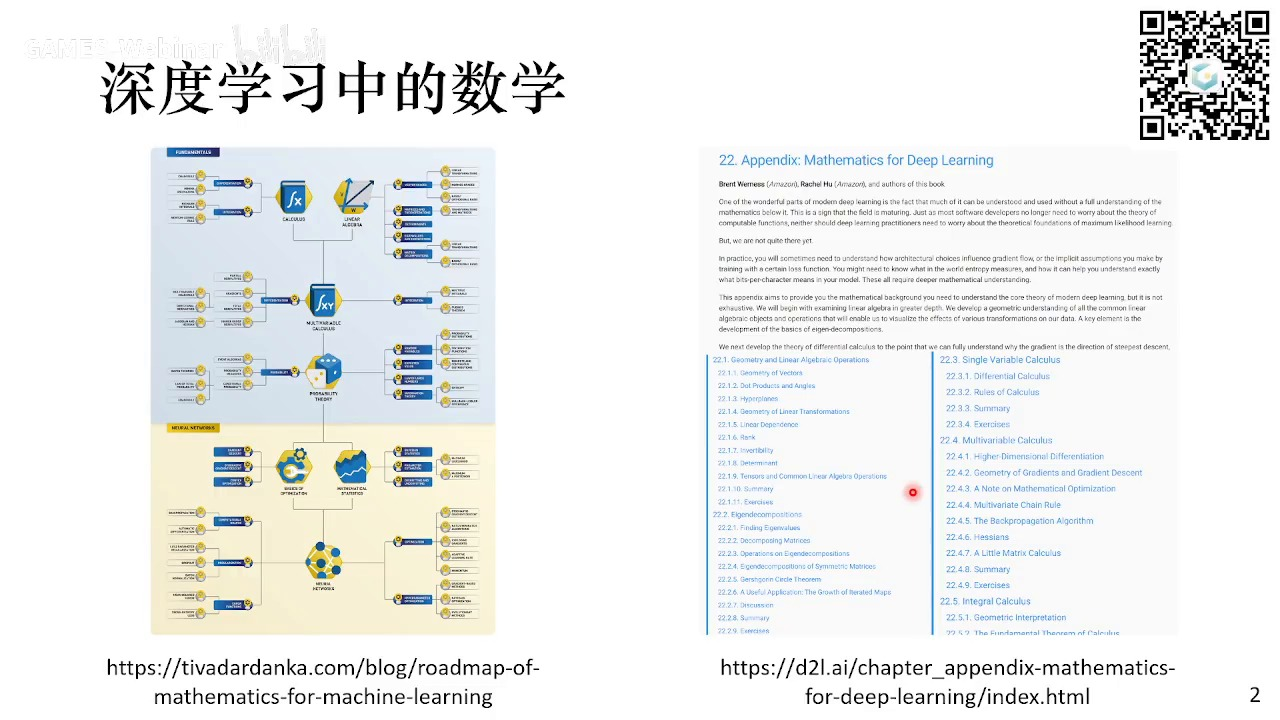
\includegraphics[width=0.92\textwidth]{figures/fig_01_roadmap.jpg}
\caption{深度学习中的数学：学习路线与参考资料\vtag}
\end{figure}
\srcnote{00:01:30--00:01:45}
\end{minipage}


本讲的路线是：先借助拟合理解深度学习；再说明生成模型的概率建模，引入 KL 散度与最大似然估计；然后详细推导变分自编码器（VAE）的损失函数，包括证据下界和重参数化；最后从 VAE 出发理解扩散模型，推导它的前向过程、反向过程和最终的损失函数。

\begin{importantbox}{本讲的主线}
生成模型要做的事，是让网络表示的分布 $\pi_\theta(x)$ 接近数据集的真实分布 $p(x)$。度量两者差距用 KL 散度，而最小化 KL 散度等价于最大似然估计。直接最大化似然算不动，于是 VAE 引入隐变量和编码器，把目标变成可计算的证据下界（ELBO）；扩散模型把一个隐变量换成一串隐变量，优化的是同一个目标，最后化简成一个非常简单的“预测噪声”的损失函数。
\end{importantbox}

\section{借助拟合理解深度学习}

\noindent\begin{minipage}{\textwidth}
\begin{figure}[H]
\centering
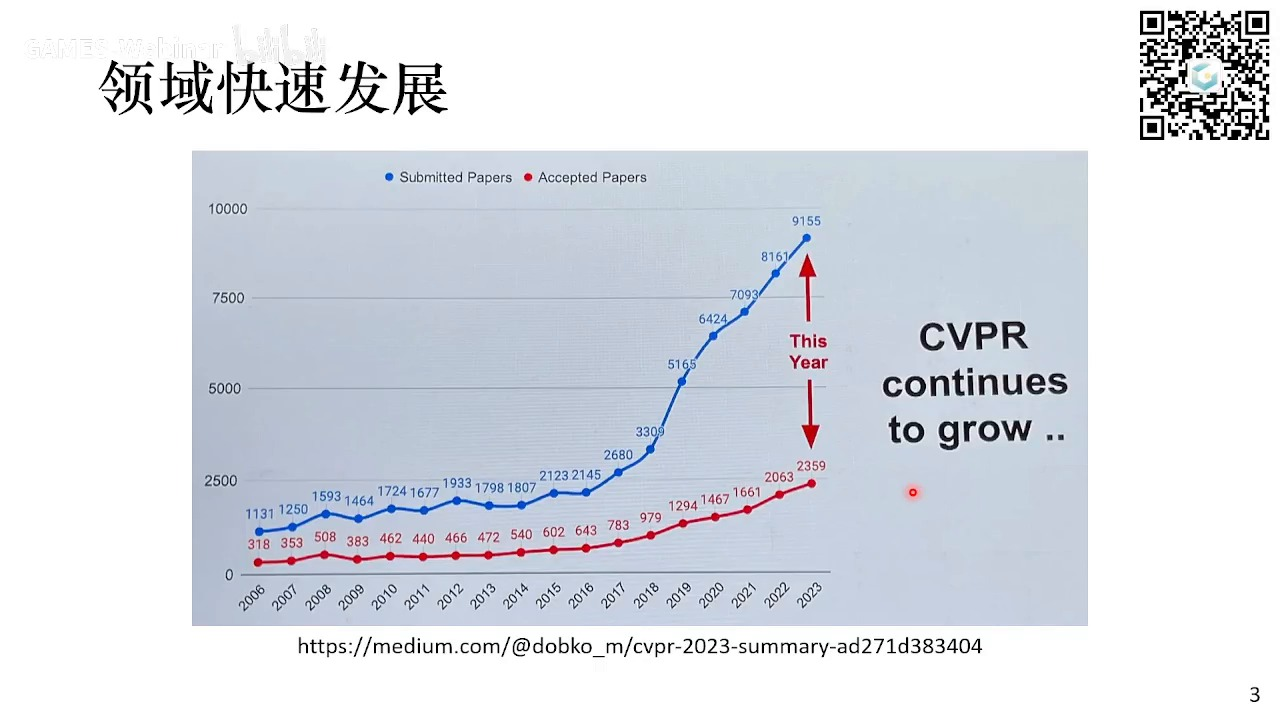
\includegraphics[width=0.92\textwidth]{figures/fig_02_growth.jpg}
\caption{领域快速发展：CVPR 投稿数量逐年增长\vtag}
\end{figure}
\srcnote{00:02:15--00:02:30}
\end{minipage}


\noindent\begin{minipage}{\textwidth}
\begin{figure}[H]
\centering
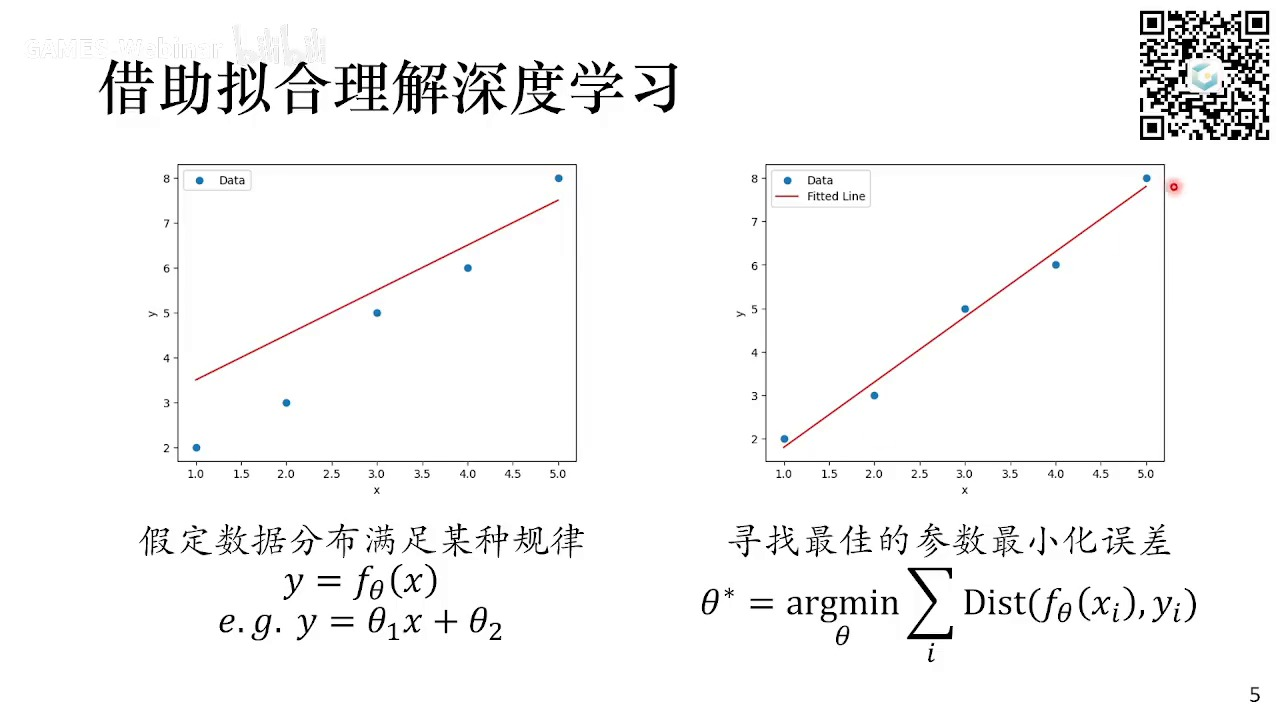
\includegraphics[width=0.92\textwidth]{figures/fig_03_fitting.jpg}
\caption{借助拟合理解深度学习：假定数据满足某种规律，再寻找最佳参数\vtag}
\end{figure}
\srcnote{00:04:30--00:04:45}
\end{minipage}


讲者从第六讲插值与拟合中的例子讲起。要对一堆散点 $(x,y)$ 做拟合，比如最简单的最小二乘拟合：先假设 $y$ 与 $x$ 之间满足某种规律 $y=f_\theta(x)$，例如 $y=\theta_1x+\theta_2$；再寻找最佳的参数，使误差最小：
\begin{equation}
\theta^*=\arg\min_\theta\sum_i\operatorname{Dist}\big(f_\theta(x_i),y_i\big).
\end{equation}

\noindent\begin{minipage}{\textwidth}
\begin{figure}[H]
\centering
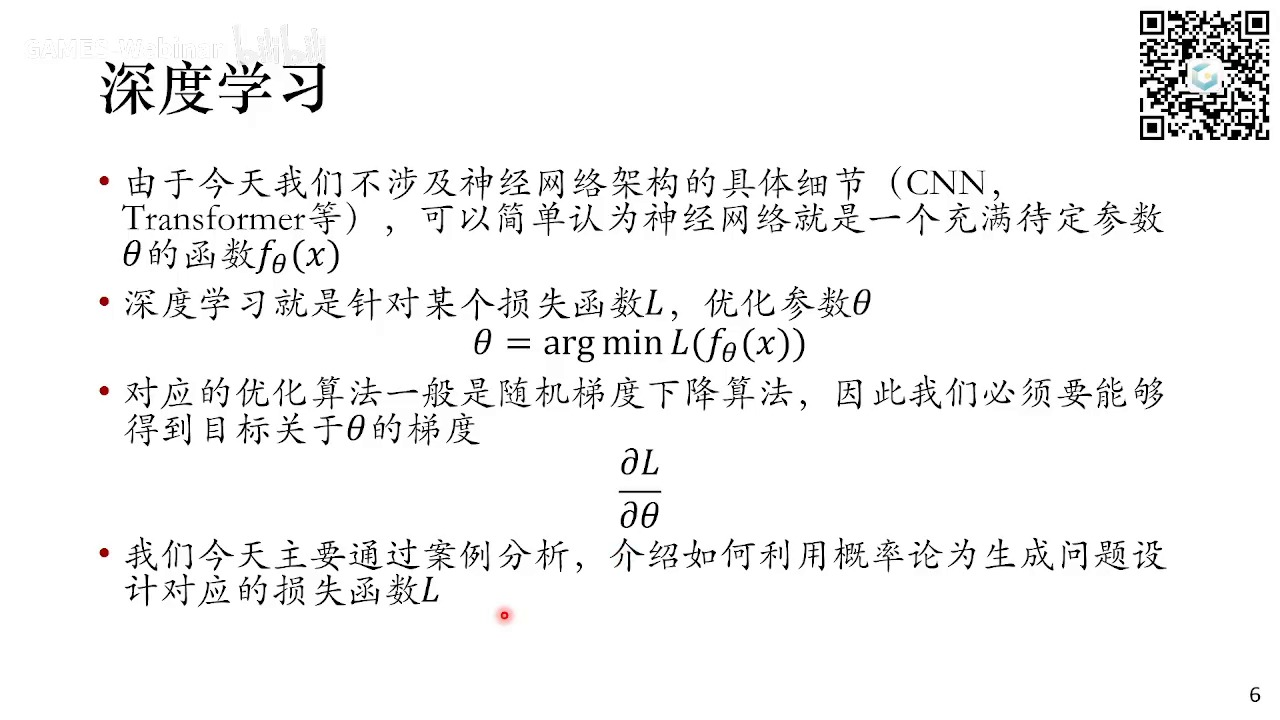
\includegraphics[width=0.92\textwidth]{figures/fig_04_deep_learning.jpg}
\caption{深度学习：针对损失函数优化网络参数\vtag}
\end{figure}
\srcnote{00:06:15--00:06:30}
\end{minipage}


深度学习本质上也是如此。由于今天不涉及神经网络架构的具体细节（CNN、Transformer 等），可以简单认为神经网络就是一个充满待定参数 $\theta$ 的函数 $f_\theta(x)$。深度学习就是针对某个具体问题定义的损失函数 $L$，优化参数 $\theta$：
\begin{equation}
\theta=\arg\min_\theta L\big(f_\theta(x)\big).
\end{equation}
对应的优化算法一般是随机梯度下降，因此必须能够得到目标关于 $\theta$ 的梯度 $\partial L/\partial\theta$。今天主要通过案例分析，介绍如何利用概率论为生成问题设计对应的损失函数 $L$。

\section{生成模型的概率建模}

\subsection{从分类到生成}

\noindent\begin{minipage}{\textwidth}
\begin{figure}[H]
\centering
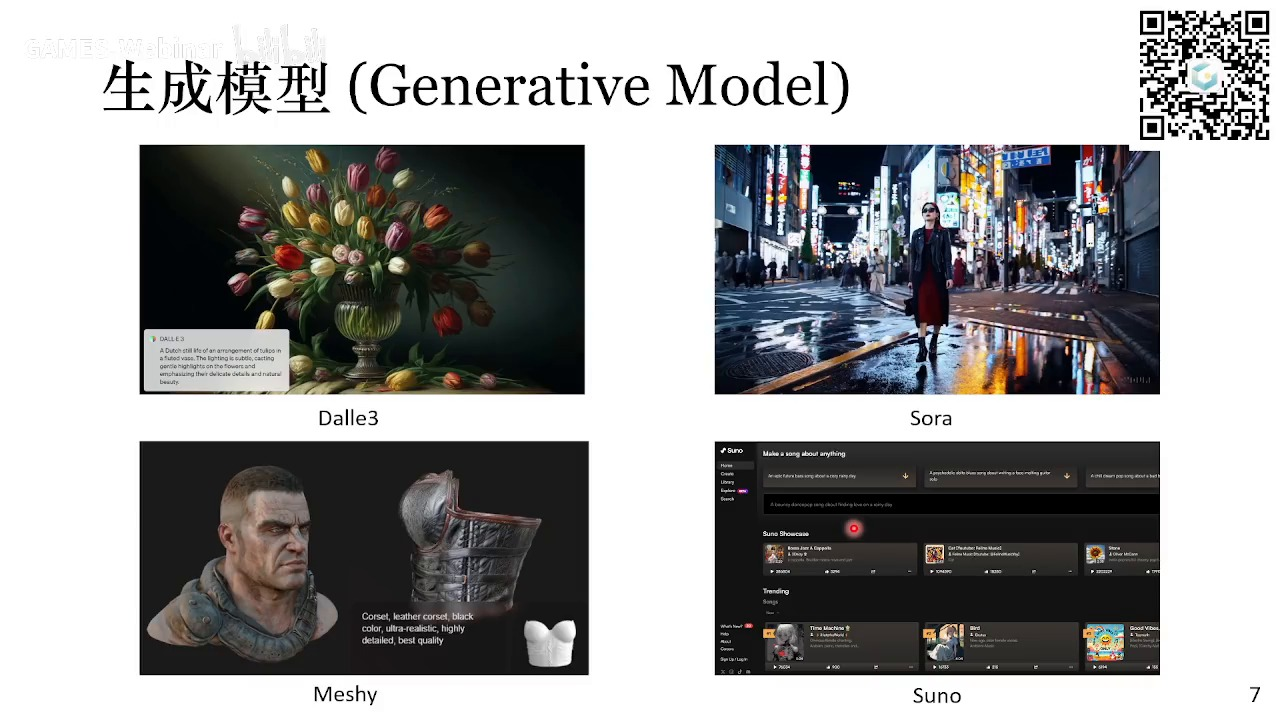
\includegraphics[width=0.92\textwidth]{figures/fig_05_generative.jpg}
\caption{生成模型的例子：DALL·E 3、Sora、Meshy 与 Suno\vtag}
\end{figure}
\srcnote{00:06:45--00:07:00}
\end{minipage}


课件展示了几个生成模型：生成图片的 DALL·E 3、生成视频的 Sora、生成三维模型的 Meshy、生成音乐的 Suno。

\noindent\begin{minipage}{\textwidth}
\begin{figure}[H]
\centering
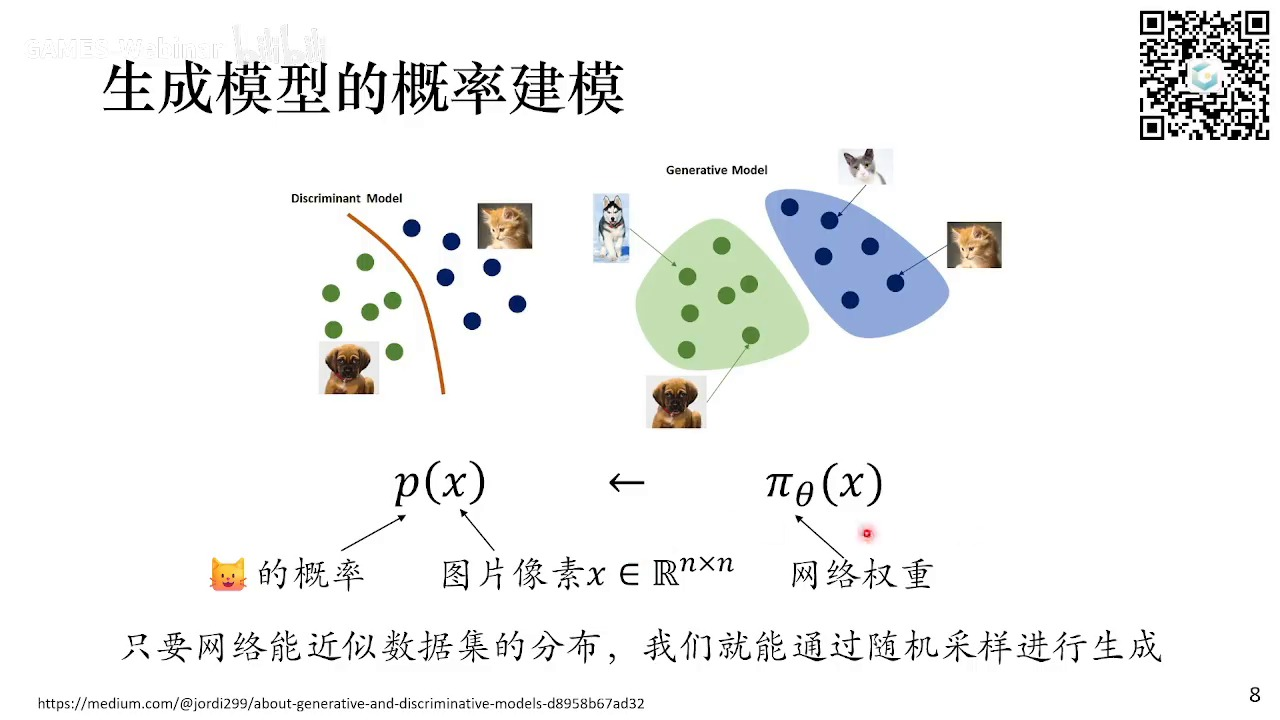
\includegraphics[width=0.92\textwidth]{figures/fig_06_prob_model.jpg}
\caption{生成模型的概率建模：数据的概率 $p(x)$ 与网络表示的 $\pi_\theta(x)$\vtag}
\end{figure}
\srcnote{00:09:00--00:09:15}
\end{minipage}


怎么理解生成模型？讲者先从大家比较熟悉的分类网络说起：给网络喂很多猫、狗、鸟的图片，它学会以后，给它一张新图片，就能告诉你这是猫还是狗。用概率的语言，假设图片的概率分布 $p(x)$ 是存在的，分类网络要做的是区分狗的概率和猫的概率，知道在哪里画一条线，线的这边是猫，那边是狗。

生成任务则是：用网络去表示数据本身的概率分布。设图片像素 $x\in\mathbb R^{n\times n}$，它的概率为 $p(x)$；网络权重为 $\theta$，网络表示的分布为 $\pi_\theta(x)$。只要网络能近似数据集的分布，就能通过随机采样进行生成：从 $\pi_\theta$ 中采样一个 $x$，它就是一张“像”数据集里的图片。

\subsection{两个问题}

\noindent\begin{minipage}{\textwidth}
\begin{figure}[H]
\centering
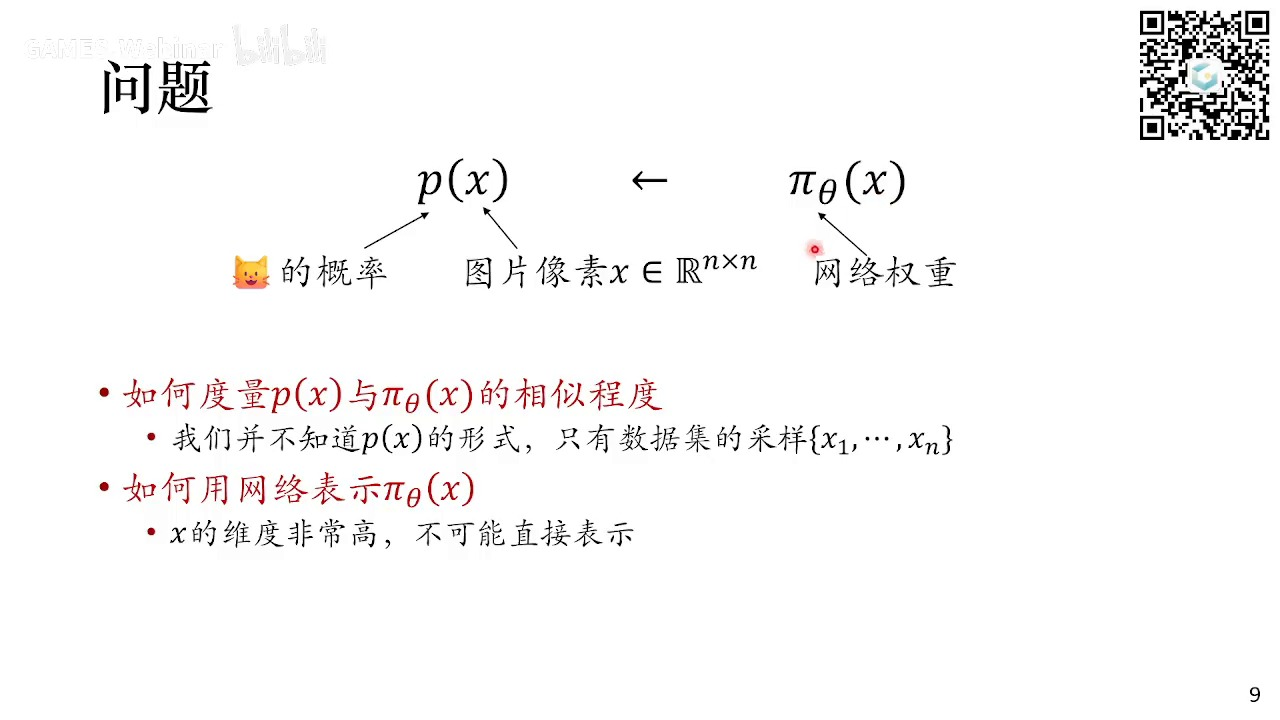
\includegraphics[width=0.92\textwidth]{figures/fig_07_problems.jpg}
\caption{生成模型面临的两个问题\vtag}
\end{figure}
\srcnote{00:10:00--00:10:15}
\end{minipage}


这样理解之后，自然有两个问题：
\begin{itemize}
\item 如何度量 $p(x)$ 与 $\pi_\theta(x)$ 的相似程度？我们并不知道 $p(x)$ 的形式，只有数据集的采样 $\{x_1,\dots,x_n\}$。
\item 如何用网络表示 $\pi_\theta(x)$？$x$ 的维度非常高，不可能直接表示。讲者举例：$512\times 512$ 像素还不算高清图片，$x$ 的维度就已经非常恐怖了，而 $\theta$ 的维度一般也很高。
\end{itemize}

\section{KL 散度与最大似然估计}

\subsection{KL 散度}

\noindent\begin{minipage}{\textwidth}
\begin{figure}[H]
\centering
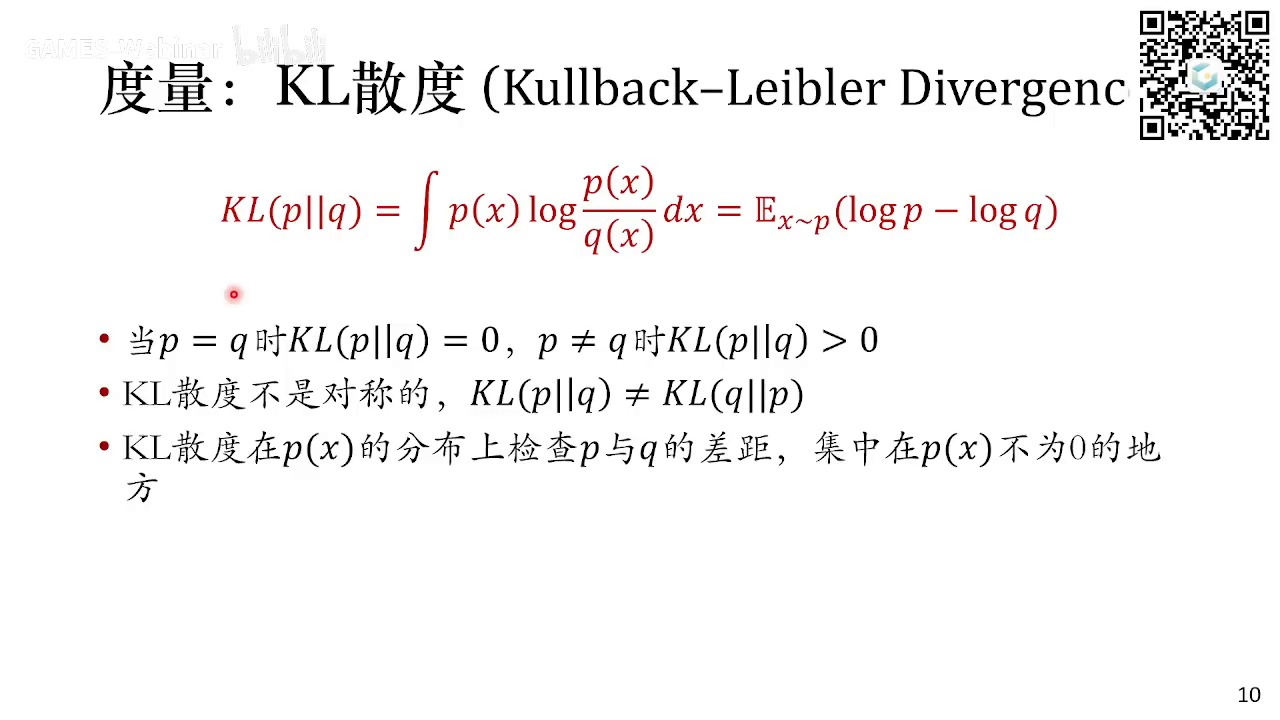
\includegraphics[width=0.92\textwidth]{figures/fig_08_kl.jpg}
\caption{度量：KL 散度的定义与性质\vtag}
\end{figure}
\srcnote{00:12:30--00:12:45}
\end{minipage}


第一个问题用 KL 散度（Kullback--Leibler divergence）来度量：
\begin{equation}
\mathrm{KL}(p\,\|\,q)=\int p(x)\log\frac{p(x)}{q(x)}\,\mathrm{d}x=\mathbb E_{x\sim p}(\log p-\log q).
\end{equation}
它有以下性质：
\begin{itemize}
\item 当 $p=q$ 时，对数里是 $\log 1=0$，所以 $\mathrm{KL}(p\|q)=0$；当 $p\ne q$ 时，可以证明 $\mathrm{KL}(p\|q)>0$。
\item KL 散度不是对称的，$\mathrm{KL}(p\|q)\ne\mathrm{KL}(q\|p)$，所以它严格来说不是距离。
\item KL 散度在 $p(x)$ 的分布上检查 $p$ 与 $q$ 的差距，集中在 $p(x)$ 不为零的地方。讲者解释：积分里乘了 $p(x)$，如果某个地方 $p(x)=0$，那里的积分贡献就为零，无论 $q$ 在那里取什么值。
\end{itemize}

\begin{knowledgebox}{为什么 KL 散度非负}
讲义作者补充：由于 $\log$ 是凹函数，由詹森不等式，$-\mathrm{KL}(p\|q)=\mathbb E_p\left[\log\frac{q}{p}\right]\le\log\mathbb E_p\left[\frac{q}{p}\right]=\log\int q\,\mathrm{d}x=\log 1=0$，等号当且仅当 $q/p$ 为常数，即 $p=q$。后面推导证据下界时会再次用到詹森不等式。
\end{knowledgebox}

\subsection{最大似然估计}

\noindent\begin{minipage}{\textwidth}
\begin{figure}[H]
\centering
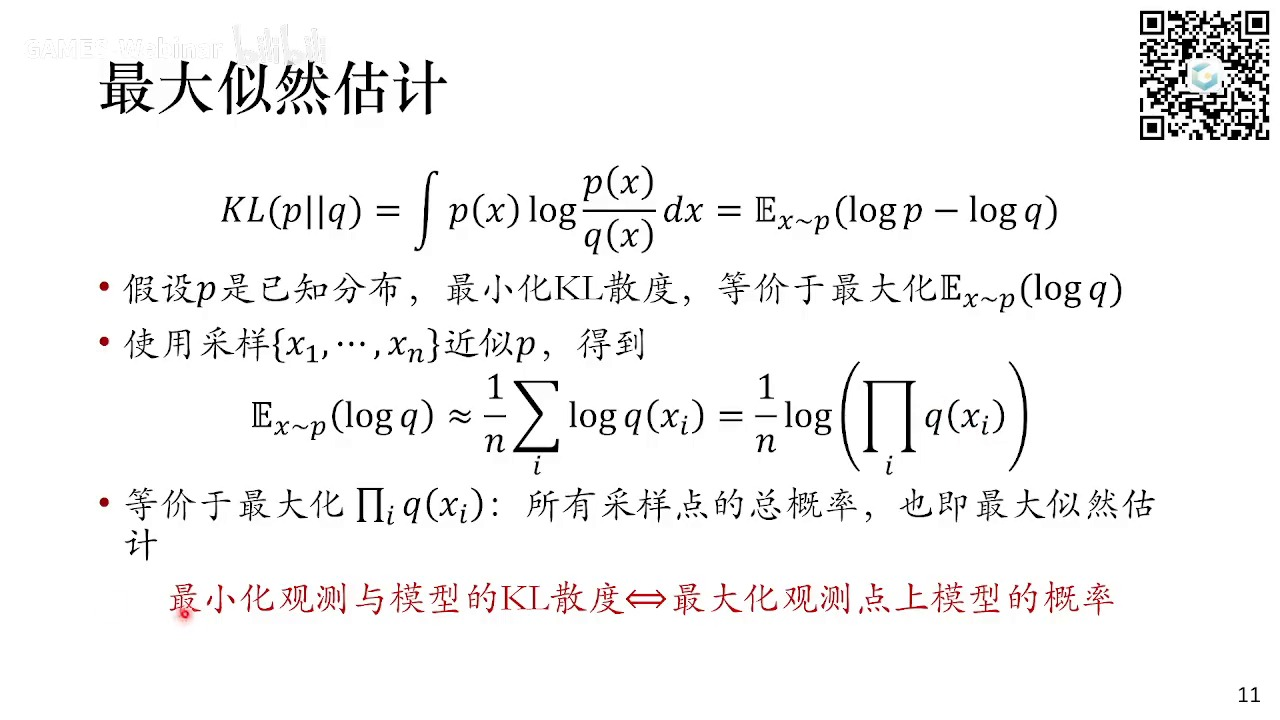
\includegraphics[width=0.92\textwidth]{figures/fig_09_mle.jpg}
\caption{最小化 KL 散度等价于最大似然估计\vtag}
\end{figure}
\srcnote{00:14:15--00:14:30}
\end{minipage}


假设 $p$ 是数据的分布（虽然未知但固定），$q$ 是要拟合的分布。由于 $\mathbb E_p(\log p)$ 与 $q$ 无关，最小化 KL 散度等价于最大化 $\mathbb E_{x\sim p}(\log q)$。用数据集的采样 $\{x_1,\dots,x_n\}$ 近似 $p$，得到
\begin{equation}
\mathbb E_{x\sim p}\log q\approx\frac{1}{n}\sum_i\log q(x_i)=\frac{1}{n}\log\prod_i q(x_i).
\end{equation}
这等价于最大化 $\prod_iq(x_i)$，即所有采样点的总概率，也就是最大似然估计。讲者概括：最小化观测与模型的 KL 散度，等价于最大化观测点上模型的概率。

\begin{warningbox}{KL 散度的方向不能随便换}
KL 散度不对称，写成 $\mathrm{KL}(p\|q)$ 时期望是对数据分布 $p$ 取的，所以只需要数据集的采样就能估计，这正是最大似然估计成立的前提。讲义作者提醒：如果反过来写成 $\mathrm{KL}(q\|p)$，期望要对模型分布取，并且需要知道 $\log p$ 的值，而 $p$ 恰恰是未知的。
\end{warningbox}


\section{变分自编码器}

\subsection{借助隐变量构造分布}

\noindent\begin{minipage}{\textwidth}
\begin{figure}[H]
\centering
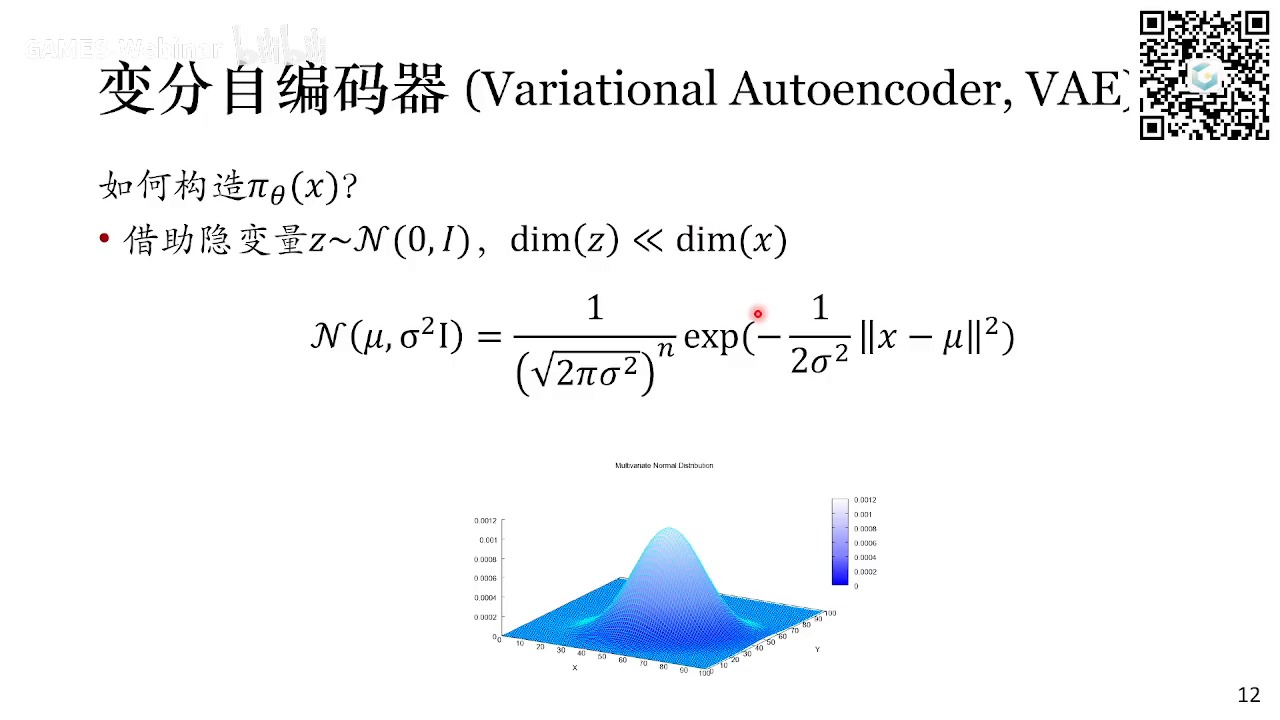
\includegraphics[width=0.92\textwidth]{figures/fig_10_vae_latent.jpg}
\caption{变分自编码器：借助低维隐变量 $z\sim\mathcal N(0,I)$\vtag}
\end{figure}
\srcnote{00:15:30--00:15:45}
\end{minipage}


第二个问题是如何构造 $\pi_\theta(x)$。变分自编码器（variational autoencoder，VAE）借助一个已知分布的隐变量 $z\sim\mathcal N(0,I)$，并且 $\dim z\ll\dim x$。课件画出的正是高维正态分布
\begin{equation}
\mathcal N(\mu,\sigma^2I)=\frac{1}{\left(\sqrt{2\pi\sigma^2}\right)^n}\exp\left(-\frac{1}{2\sigma^2}\|x-\mu\|^2\right).
\end{equation}

\noindent\begin{minipage}{\textwidth}
\begin{figure}[H]
\centering
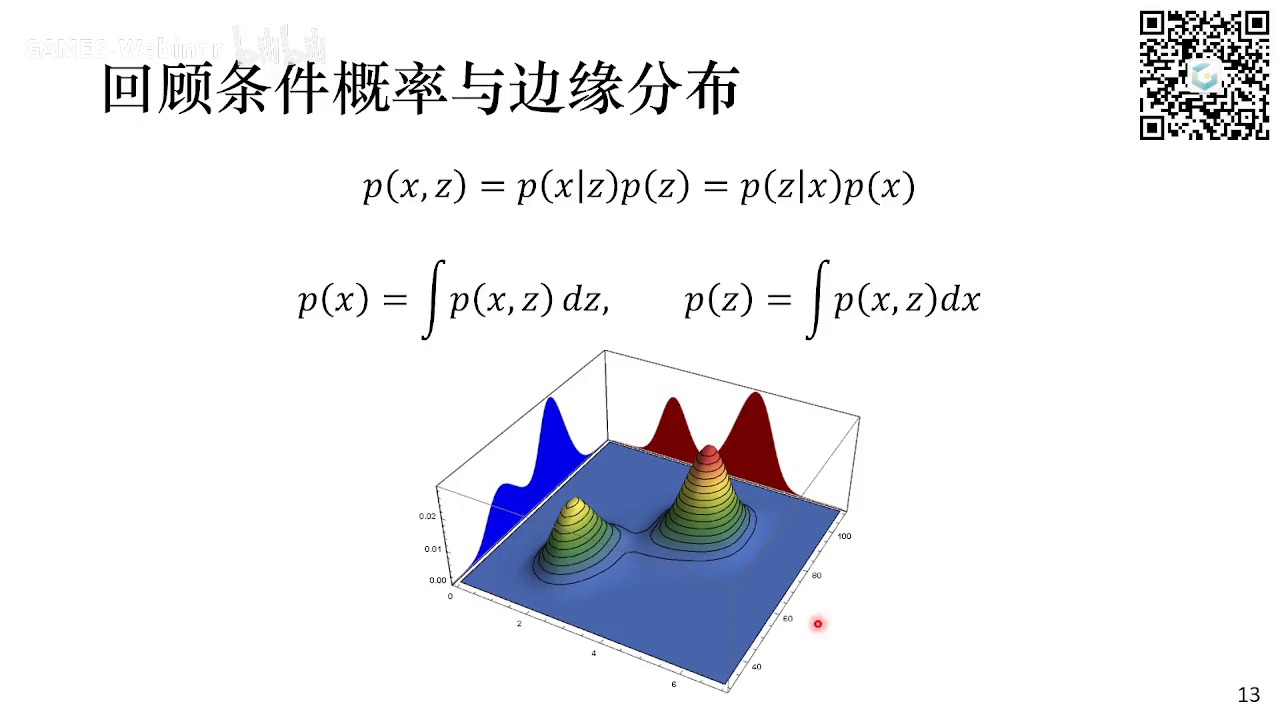
\includegraphics[width=0.92\textwidth]{figures/fig_11_conditional.jpg}
\caption{回顾条件概率与边缘分布\vtag}
\end{figure}
\srcnote{00:16:45--00:17:00}
\end{minipage}


讲者回顾了第八讲的条件概率与边缘分布：联合概率可以先有 $p(z)$ 再乘以条件概率 $p(x\mid z)$，也可以先有 $p(x)$ 再乘以 $p(z\mid x)$，
\begin{equation}
p(x,z)=p(x\mid z)p(z)=p(z\mid x)p(x),\qquad p(x)=\int p(x,z)\,\mathrm{d}z,\quad p(z)=\int p(x,z)\,\mathrm{d}x .
\end{equation}

\noindent\begin{minipage}{\textwidth}
\begin{figure}[H]
\centering
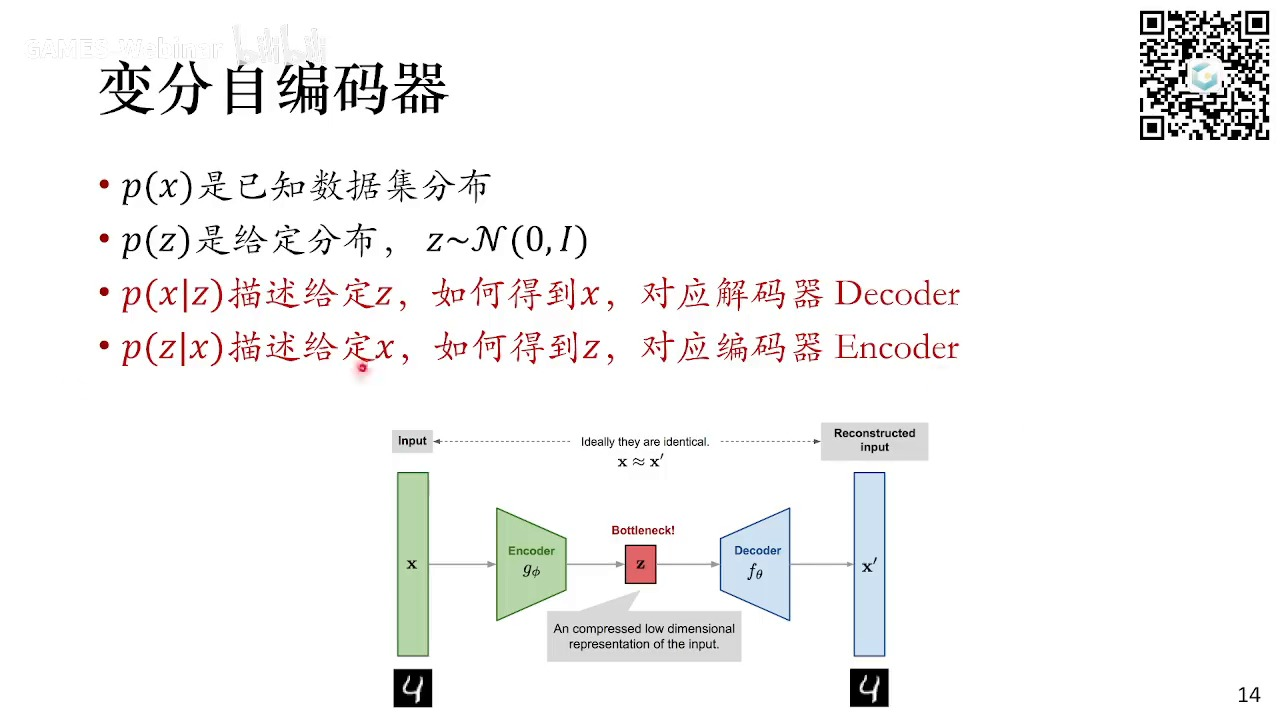
\includegraphics[width=0.92\textwidth]{figures/fig_12_vae_roles.jpg}
\caption{VAE 中各个概率的含义：编码器与解码器\vtag}
\end{figure}
\srcnote{00:18:00--00:18:15}
\end{minipage}


在 VAE 中：$p(x)$ 是已知的数据集分布（只有采样）；$p(z)$ 是给定的分布，$z\sim\mathcal N(0,I)$；$p(x\mid z)$ 描述给定 $z$ 如何得到 $x$，对应解码器（decoder）；$p(z\mid x)$ 描述给定 $x$ 如何得到 $z$，对应编码器（encoder）。

\subsection{为什么需要编码器}

\noindent\begin{minipage}{\textwidth}
\begin{figure}[H]
\centering
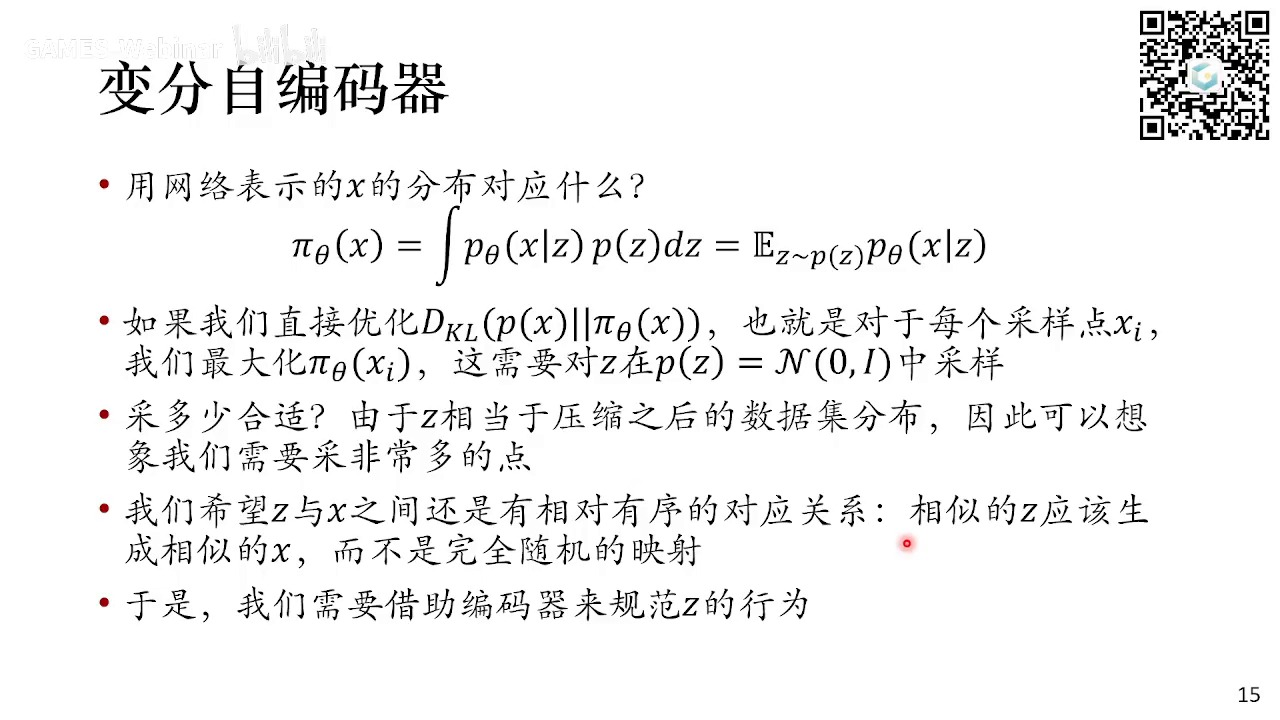
\includegraphics[width=0.92\textwidth]{figures/fig_13_vae_why_encoder.jpg}
\caption{直接优化的困难与引入编码器的动机\vtag}
\end{figure}
\srcnote{00:20:30--00:20:45}
\end{minipage}


用网络表示的 $x$ 的分布是
\begin{equation}
\pi_\theta(x)=\int p_\theta(x\mid z)p(z)\,\mathrm{d}z=\mathbb E_{z\sim p(z)}\,p_\theta(x\mid z).
\end{equation}
如果直接优化 $D_{\mathrm{KL}}(p(x)\|\pi_\theta(x))$，即对每个采样点 $x_i$ 最大化 $\pi_\theta(x_i)$，就需要对 $z$ 在 $p(z)=\mathcal N(0,I)$ 中采样来求期望。讲者问：采多少合适？由于 $z$ 相当于压缩之后的数据集分布，可以想象需要采非常非常多的点，这基本上是不可计算的。所以就算数学形式上很漂亮，只要优化 KL 散度就可以，但实际不可操作。

另外，我们希望 $z$ 与 $x$ 之间有相对有序的对应关系：相似的 $z$ 应该生成相似的 $x$，而不是完全随机的映射。于是需要借助编码器来规范 $z$ 的行为，让我们知道每个 $x$ 大概对应哪里的 $z$，从而减少采样。

\begin{importantbox}{编码器解决的是采样效率问题}
直接对 $p(z)=\mathcal N(0,I)$ 采样时，绝大多数 $z$ 解码出来与当前数据点 $x_i$ 毫不相关，对 $\pi_\theta(x_i)$ 的贡献几乎为零。编码器 $q_\phi(z\mid x_i)$ 先告诉我们 $x_i$ 大概对应哪一小片 $z$，只在那里采样，期望就能用很少的样本估计。
\end{importantbox}


\subsection{两个网络}

\noindent\begin{minipage}{\textwidth}
\begin{figure}[H]
\centering
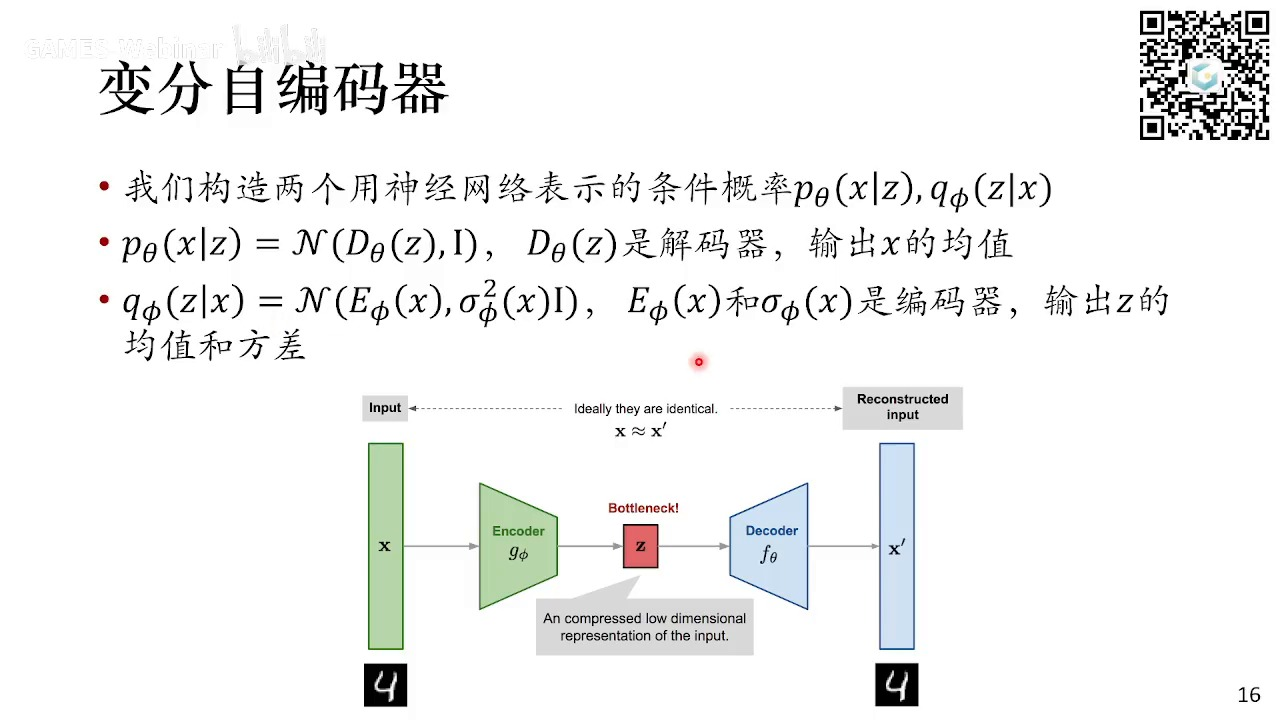
\includegraphics[width=0.92\textwidth]{figures/fig_14_vae_networks.jpg}
\caption{用神经网络表示的两个条件概率\vtag}
\end{figure}
\srcnote{00:22:15--00:22:30}
\end{minipage}


构造两个用神经网络表示的条件概率：
\begin{equation}
p_\theta(x\mid z)=\mathcal N\big(D_\theta(z),I\big),\qquad q_\phi(z\mid x)=\mathcal N\big(E_\phi(x),\sigma_\phi^2(x)I\big).
\end{equation}
$D_\theta(z)$ 是解码器，输出 $x$ 的均值；$E_\phi(x)$ 和 $\sigma_\phi(x)$ 是编码器，输出 $z$ 的均值和方差。讲者解释：编码器拿到一个很长维度的 $x$，输出两个东西，均值和方差，它们一起确定一个正态分布。

于是有两种方式表达 $x$ 与 $z$ 的联合分布：
\begin{equation}
p(x,z)=p_\theta(x\mid z)p(z),\qquad q(x,z)=q_\phi(z\mid x)p(x),
\end{equation}
一个从解码器方向来，一个从编码器方向来。我们转而优化二者的 KL 散度 $D_{\mathrm{KL}}\big(q(x,z)\,\|\,p(x,z)\big)$。

\section{VAE 的损失函数}

\subsection{展开 KL 散度}

\noindent\begin{minipage}{\textwidth}
\begin{figure}[H]
\centering
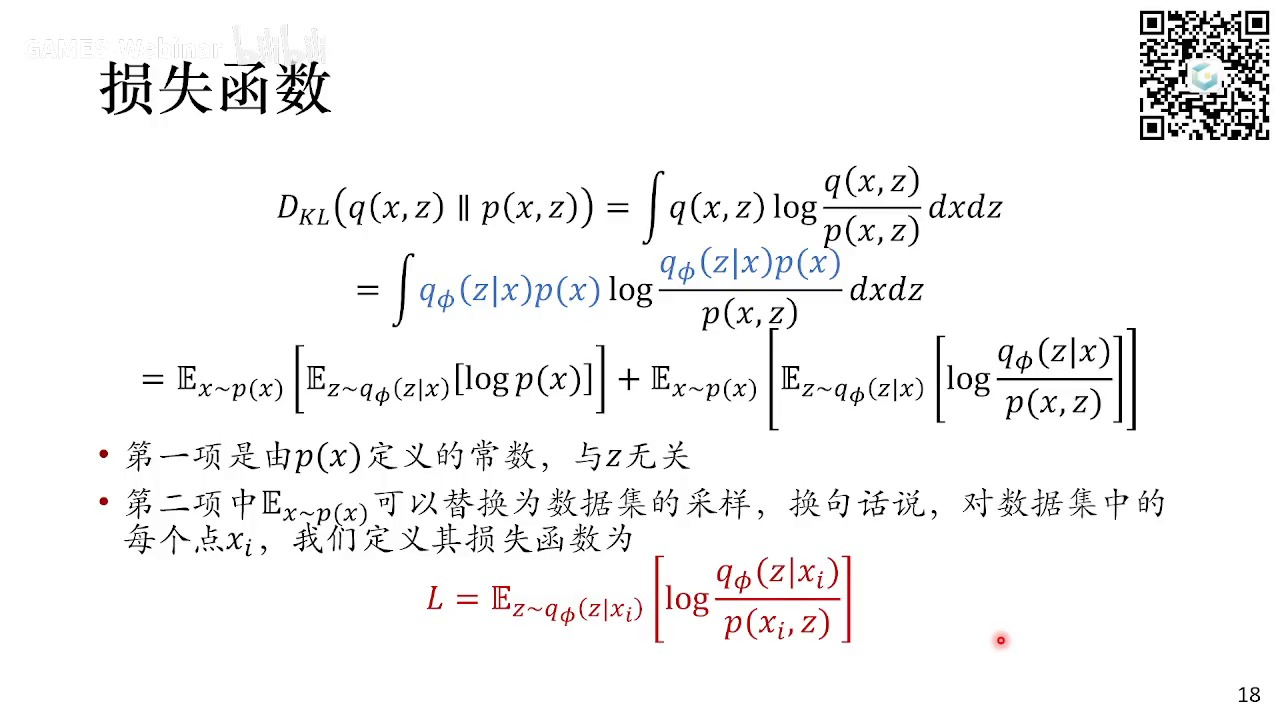
\includegraphics[width=0.92\textwidth]{figures/fig_15_vae_loss1.jpg}
\caption{VAE 损失函数的推导：展开联合分布的 KL 散度\vtag}
\end{figure}
\srcnote{00:26:30--00:26:45}
\end{minipage}


展开后，把所有涉及 $p(x)$ 的积分写成关于 $p$ 分布的期望：
\begin{equation}
\begin{aligned}
D_{\mathrm{KL}}\big(q(x,z)\|p(x,z)\big)&=\iint q_\phi(z\mid x)p(x)\log\frac{q_\phi(z\mid x)p(x)}{p(x,z)}\,\mathrm{d}x\,\mathrm{d}z\\
&=\mathbb E_{x\sim p(x)}\mathbb E_{z\sim q_\phi(z\mid x)}\log p(x)+\mathbb E_{x\sim p(x)}\mathbb E_{z\sim q_\phi(z\mid x)}\log\frac{q_\phi(z\mid x)}{p(x,z)} .
\end{aligned}
\end{equation}
第一项是由 $p(x)$ 定义的常数，与网络参数和 $z$ 都无关；第二项中 $\mathbb E_{x\sim p(x)}$ 可以替换为数据集的采样。换句话说，对数据集中的每个点 $x_i$，定义其损失函数为
\begin{equation}
L=\mathbb E_{z\sim q_\phi(z\mid x_i)}\log\frac{q_\phi(z\mid x_i)}{p(x_i,z)} .
\end{equation}
对每个 $x_i$ 求出 $L$，把梯度回传到网络参数，就可以训练。

\subsection{证据下界}

\noindent\begin{minipage}{\textwidth}
\begin{figure}[H]
\centering
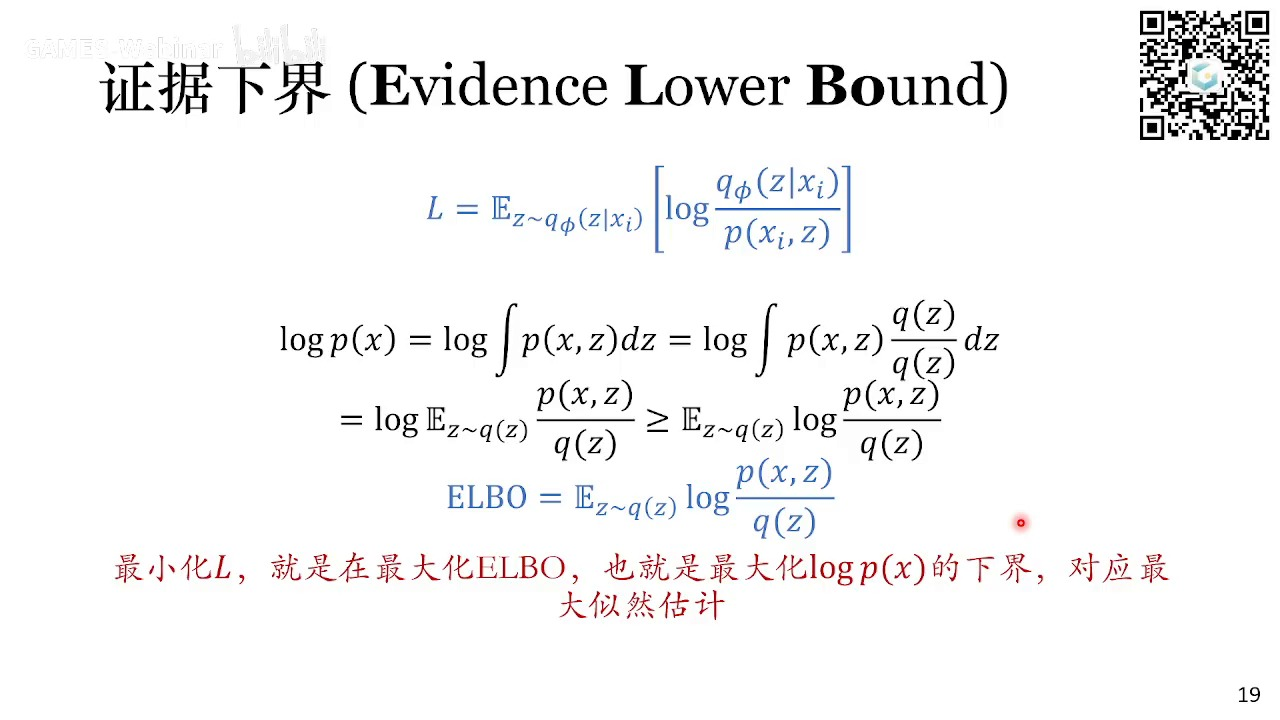
\includegraphics[width=0.92\textwidth]{figures/fig_16_elbo.jpg}
\caption{证据下界（ELBO）与最大似然估计的关系\vtag}
\end{figure}
\srcnote{00:29:15--00:29:30}
\end{minipage}


讲者又给出了理解这个损失函数的另一种方式。对任意分布 $q(z)$，
\begin{equation}
\log p(x)=\log\int p(x,z)\,\mathrm{d}z=\log\int q(z)\frac{p(x,z)}{q(z)}\,\mathrm{d}z=\log\mathbb E_{z\sim q(z)}\frac{p(x,z)}{q(z)}\ge\mathbb E_{z\sim q(z)}\log\frac{p(x,z)}{q(z)} .
\end{equation}
最后一步是詹森不等式。右边定义为证据下界（evidence lower bound，ELBO）：
\begin{equation}
\mathrm{ELBO}=\mathbb E_{z\sim q(z)}\log\frac{p(x,z)}{q(z)} .
\end{equation}
对比可以发现，损失函数 $L$ 恰好是 ELBO 的相反数，只是对数里的分子分母交换了一下。所以最小化 $L$，就是在最大化 ELBO，也就是最大化 $\log p(x)$ 的下界，对应最大似然估计，与最开始的理解一致。

\begin{knowledgebox}{下界差了多少}
讲义作者补充：利用 $p(x,z)=p(z\mid x)p(x)$ 可以直接算出 $\log p(x)-\mathrm{ELBO}=D_{\mathrm{KL}}\big(q(z)\,\|\,p(z\mid x)\big)\ge 0$。所以当 $q(z)$ 恰好等于真实后验 $p(z\mid x)$ 时下界是紧的；编码器 $q_\phi(z\mid x)$ 越接近真实后验，最大化 ELBO 就越接近真正的最大似然。
\end{knowledgebox}


\subsection{拆成两项}

\noindent\begin{minipage}{\textwidth}
\begin{figure}[H]
\centering
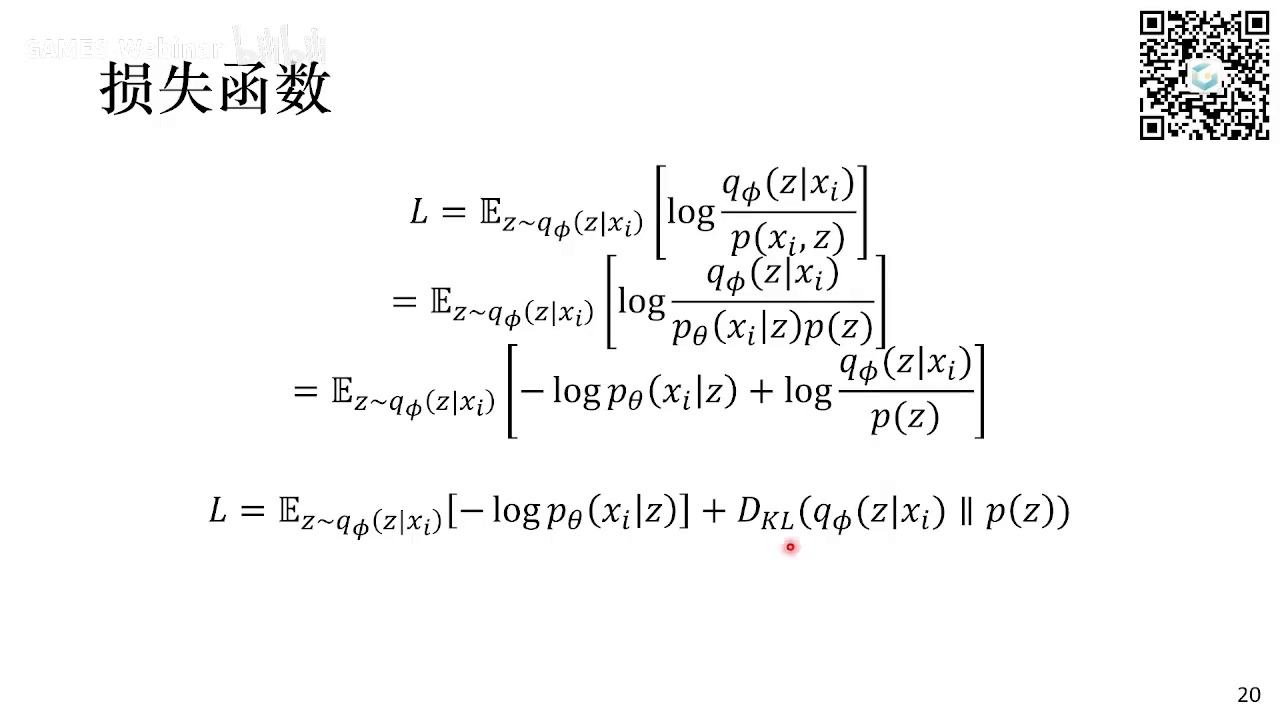
\includegraphics[width=0.92\textwidth]{figures/fig_17_vae_loss2.jpg}
\caption{损失函数拆成重建项与 KL 项\vtag}
\end{figure}
\srcnote{00:30:00--00:30:15}
\end{minipage}


把 $p(x_i,z)=p_\theta(x_i\mid z)p(z)$ 代入：
\begin{equation}
L=\mathbb E_{z\sim q_\phi(z\mid x_i)}\left[-\log p_\theta(x_i\mid z)+\log\frac{q_\phi(z\mid x_i)}{p(z)}\right]=\mathbb E_{z\sim q_\phi(z\mid x_i)}\big[-\log p_\theta(x_i\mid z)\big]+D_{\mathrm{KL}}\big(q_\phi(z\mid x_i)\,\|\,p(z)\big).
\end{equation}
第二项的期望里是 $\log(q/p)$，正好是 KL 散度的定义。

\subsection{第一项：重建误差}

\noindent\begin{minipage}{\textwidth}
\begin{figure}[H]
\centering
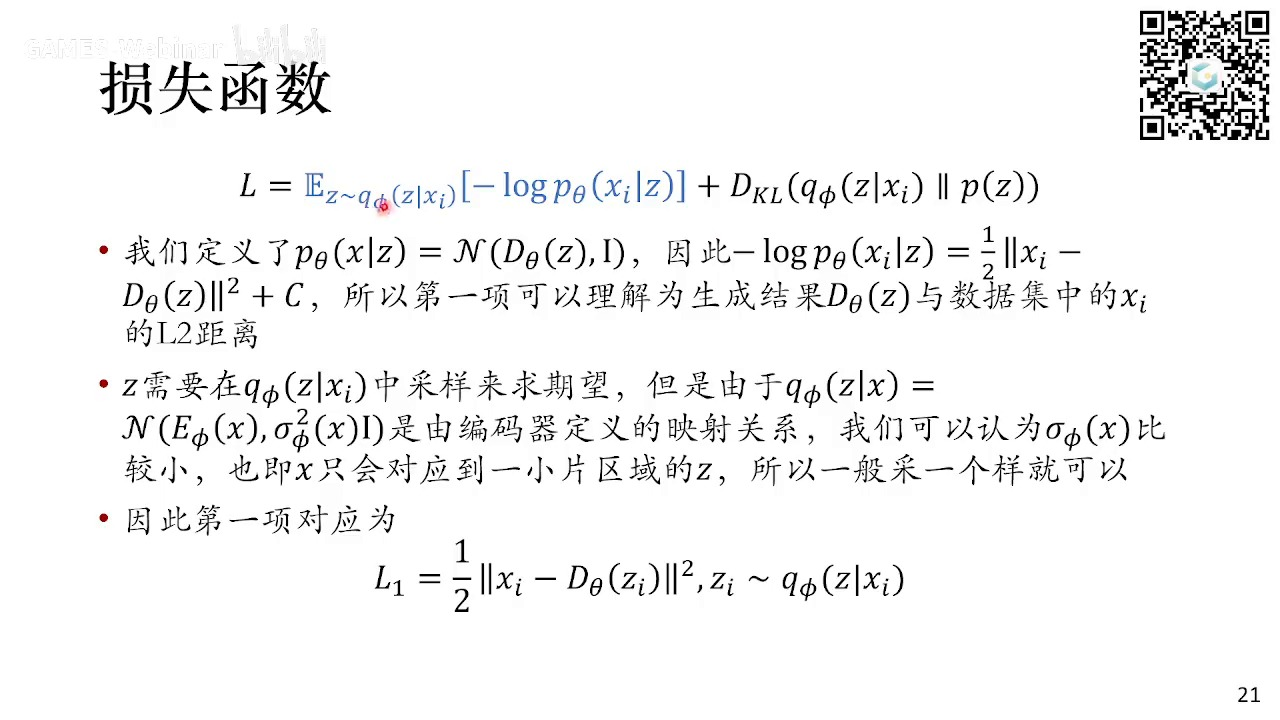
\includegraphics[width=0.92\textwidth]{figures/fig_18_vae_term1.jpg}
\caption{第一项：生成结果与数据点的 L2 距离\vtag}
\end{figure}
\srcnote{00:31:30--00:31:45}
\end{minipage}


由于定义了 $p_\theta(x\mid z)=\mathcal N(D_\theta(z),I)$，代入正态分布的密度，
\begin{equation}
-\log p_\theta(x_i\mid z)=\frac{1}{2}\|x_i-D_\theta(z)\|^2+C,
\end{equation}
所以第一项可以理解为生成结果 $D_\theta(z)$ 与数据集中 $x_i$ 的 L2 距离。讲者说这很好理解：当然希望生成结果与数据集足够接近。

$z$ 需要在 $q_\phi(z\mid x_i)$ 中采样来求期望。和前面不同的是，这里 $z$ 的分布是编码器的输出：给它数据集里的点 $x_i$，它吐出均值和方差。可以认为 $\sigma_\phi(x)$ 比较小，也即 $x$ 只会对应到一小片区域的 $z$，所以一般采一个样就可以。因此第一项对应为
\begin{equation}
L_1=\frac{1}{2}\|x_i-D_\theta(z_i)\|^2,\qquad z_i\sim q_\phi(z\mid x_i).
\end{equation}

\subsection{重参数化}

\noindent\begin{minipage}{\textwidth}
\begin{figure}[H]
\centering
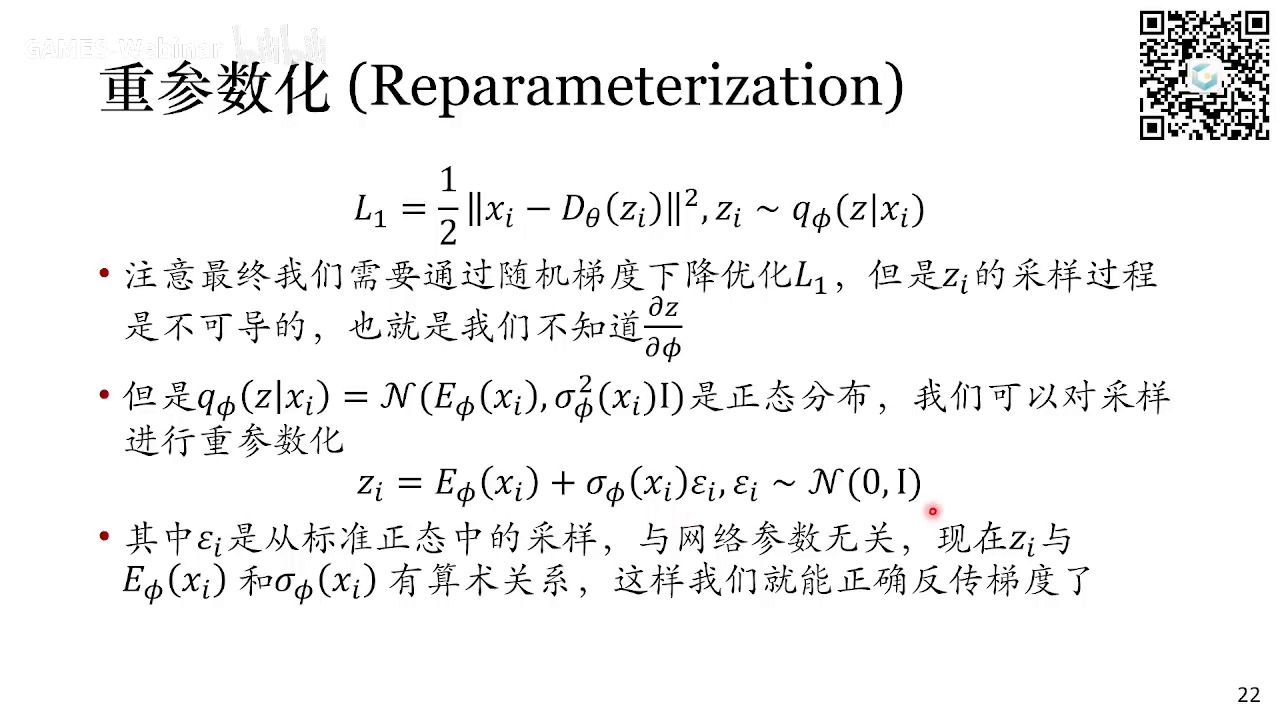
\includegraphics[width=0.92\textwidth]{figures/fig_19_reparam.jpg}
\caption{重参数化技巧：让采样过程可以反传梯度\vtag}
\end{figure}
\srcnote{00:35:45--00:36:00}
\end{minipage}


最终要通过随机梯度下降优化 $L_1$，但 $z_i$ 的采样过程是不可导的，也就是不知道 $\partial L/\partial\phi$。讲者说，这其实并不直接，但也很好理解：$q_\phi(z\mid x_i)=\mathcal N(E_\phi(x_i),\sigma_\phi^2(x_i)I)$ 是正态分布，可以对采样进行重参数化：
\begin{equation}
z_i=E_\phi(x_i)+\sigma_\phi(x_i)\varepsilon_i,\qquad \varepsilon_i\sim\mathcal N(0,I).
\end{equation}
其中 $\varepsilon_i$ 是从标准正态中的采样，与网络参数无关。可以直接理解成：把标准高斯分布做了一下平移和缩放，变成想要的高斯分布，这与直接从 $q_\phi$ 中采样的结果是一样的。现在 $z_i$ 与 $E_\phi(x_i)$、$\sigma_\phi(x_i)$ 有算术关系，就能正确反传梯度了。

\begin{importantbox}{重参数化的要点}
重参数化把“随机性”从依赖参数的分布里挪出来，放进一个与参数无关的噪声 $\varepsilon$ 中。这样随机节点不再挡在梯度路径上，梯度可以穿过 $z=\mu+\sigma\varepsilon$ 这个确定的算术运算流向编码器。后面扩散模型的前向过程会反复用到同一个技巧。
\end{importantbox}

\subsection{第二项：KL 正则}

\noindent\begin{minipage}{\textwidth}
\begin{figure}[H]
\centering
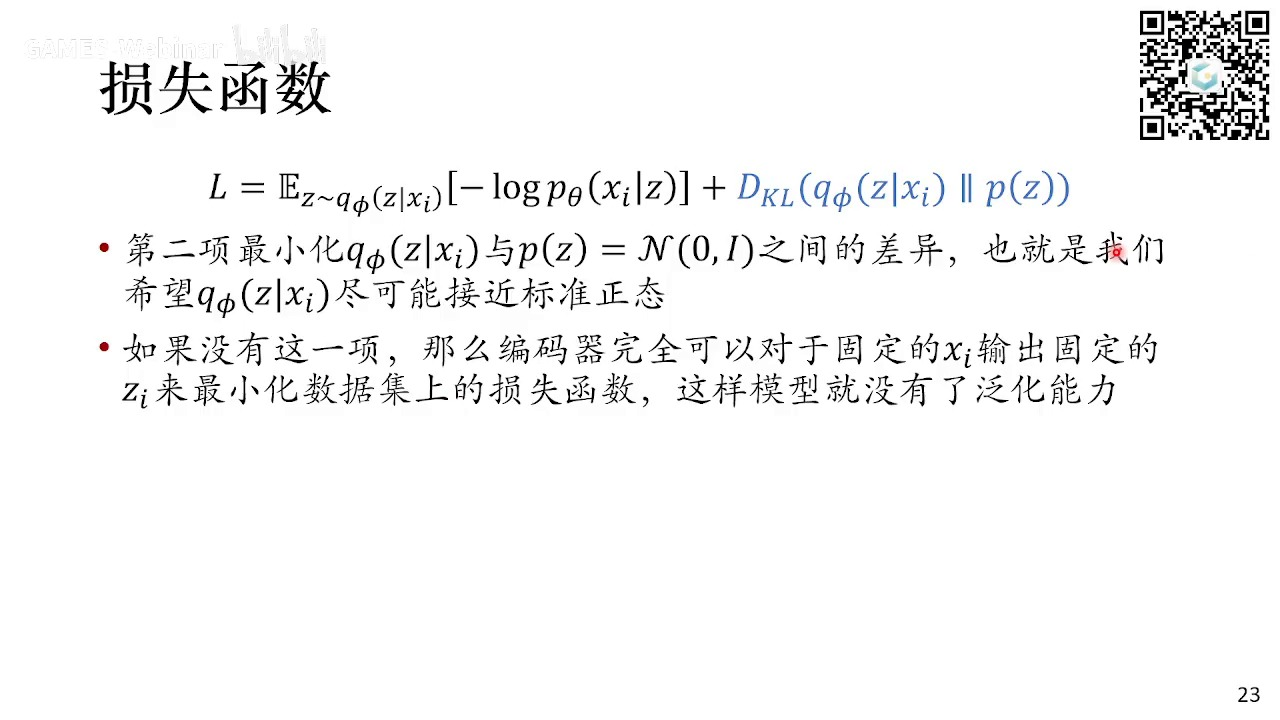
\includegraphics[width=0.92\textwidth]{figures/fig_20_vae_term2.jpg}
\caption{第二项：让编码器的分布接近标准正态\vtag}
\end{figure}
\srcnote{00:38:00--00:38:15}
\end{minipage}


第二项最小化 $q_\phi(z\mid x_i)$ 与 $p(z)=\mathcal N(0,I)$ 之间的差异，也就是希望编码器给出的分布尽可能接近标准正态。如果没有这一项，编码器完全可以对固定的 $x_i$ 输出固定的 $z_i$ 来最小化数据集上的损失函数。讲者解释，那样它很可能把数据集里那些点都重建得很像，但如果要它生成新的东西，就没办法了，模型没有了泛化能力。第二项让 $z$ 的分布铺满标准正态，而不是过拟合到数据集的那些点上。

\noindent\begin{minipage}{\textwidth}
\begin{figure}[H]
\centering
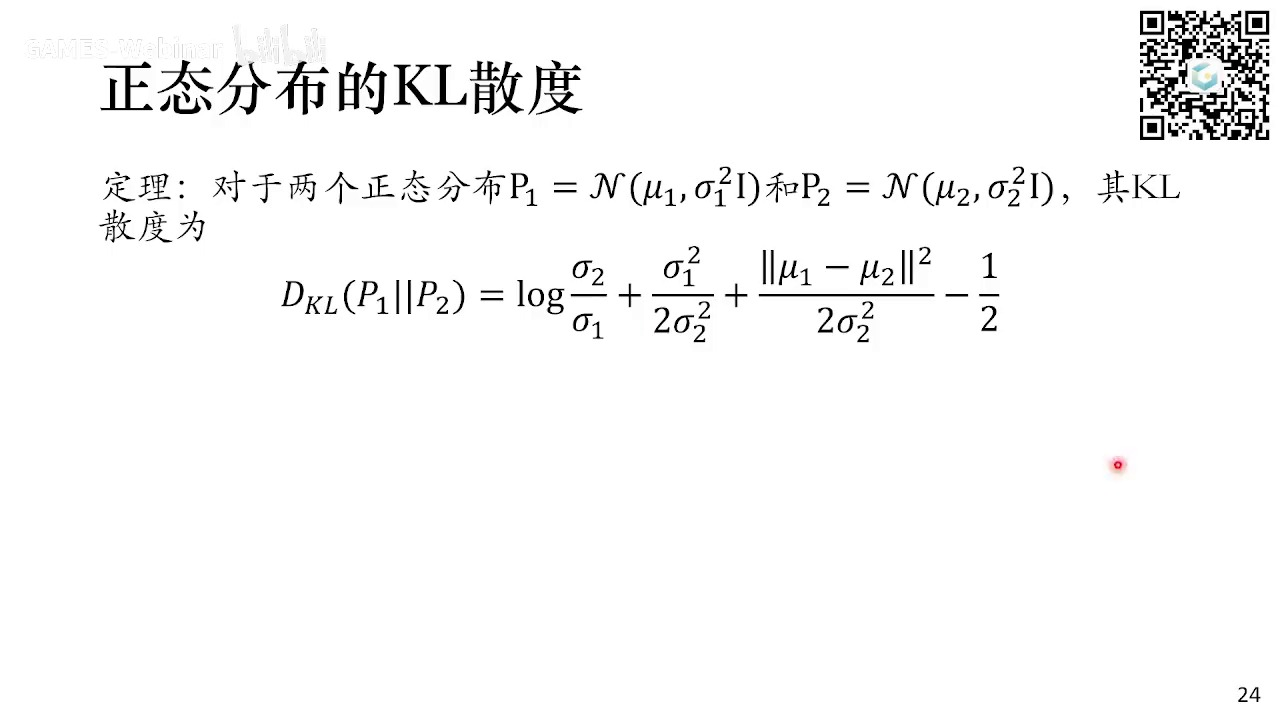
\includegraphics[width=0.92\textwidth]{figures/fig_21_gauss_kl.jpg}
\caption{两个正态分布的 KL 散度\vtag}
\end{figure}
\srcnote{00:38:30--00:38:45}
\end{minipage}


对两个正态分布 $P_1=\mathcal N(\mu_1,\sigma_1^2I)$ 和 $P_2=\mathcal N(\mu_2,\sigma_2^2I)$，KL 散度有解析表达式。课件给出的一维形式为
\begin{equation}
D_{\mathrm{KL}}(P_1\|P_2)=\log\frac{\sigma_2}{\sigma_1}+\frac{\sigma_1^2+(\mu_1-\mu_2)^2}{2\sigma_2^2}-\frac{1}{2} .
\end{equation}

\begin{warningbox}{高维时要乘以维数}
课件上的式子是一维的情形。讲义作者提醒：对 $d$ 维各向同性高斯，前一项和最后一项都要乘以 $d$，方差项也变成 $d\sigma_1^2$，即 $D_{\mathrm{KL}}=d\log\frac{\sigma_2}{\sigma_1}+\frac{d\sigma_1^2+\|\mu_1-\mu_2\|^2}{2\sigma_2^2}-\frac{d}{2}$。下面 $L_2$ 中出现的 $d$ 正是由此而来。
\end{warningbox}

\noindent\begin{minipage}{\textwidth}
\begin{figure}[H]
\centering
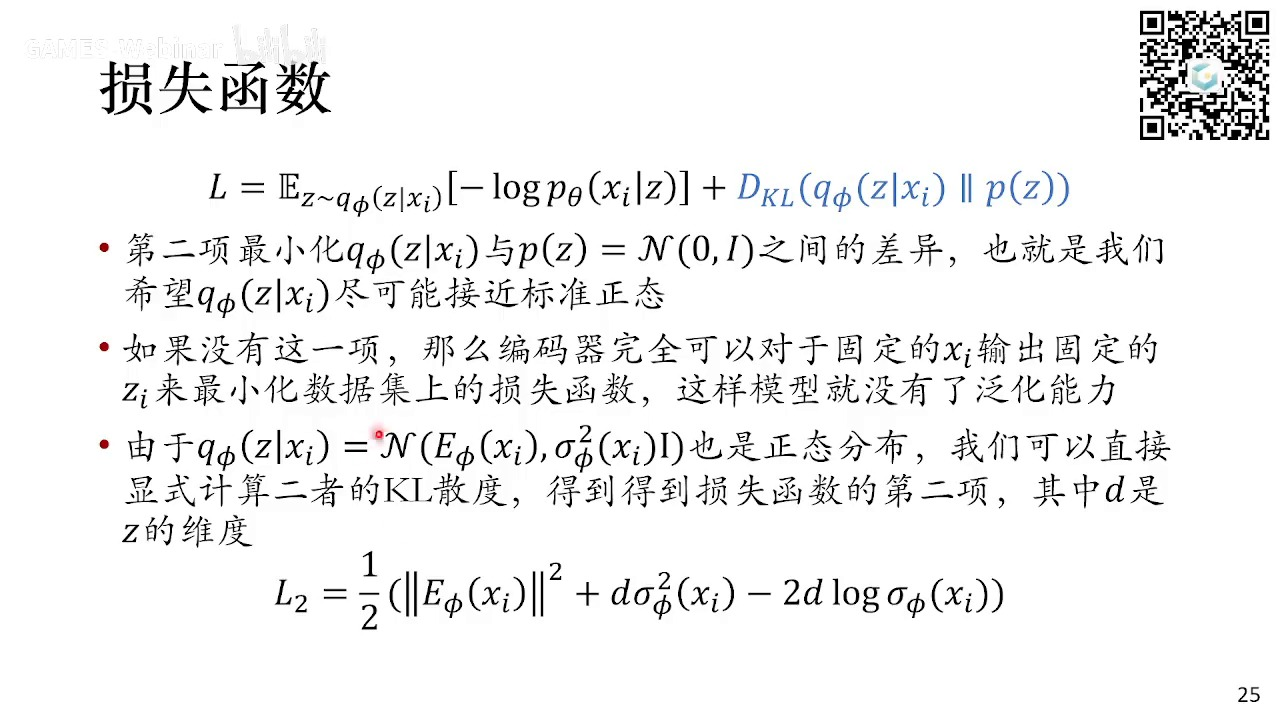
\includegraphics[width=0.92\textwidth]{figures/fig_22_vae_term2_final.jpg}
\caption{第二项的显式形式\vtag}
\end{figure}
\srcnote{00:38:45--00:39:00}
\end{minipage}


由于 $q_\phi(z\mid x_i)$ 也是正态分布，可以直接显式计算它与标准正态的 KL 散度。取 $\mu_2=0$，$\sigma_2=1$，略去常数，得到损失函数的第二项，其中 $d$ 是 $z$ 的维度：
\begin{equation}
L_2=\frac{1}{2}\left(\|E_\phi(x_i)\|^2+d\sigma_\phi^2(x_i)-2d\log\sigma_\phi(x_i)\right).
\end{equation}

\subsection{训练与生成}

\noindent\begin{minipage}{\textwidth}
\begin{figure}[H]
\centering
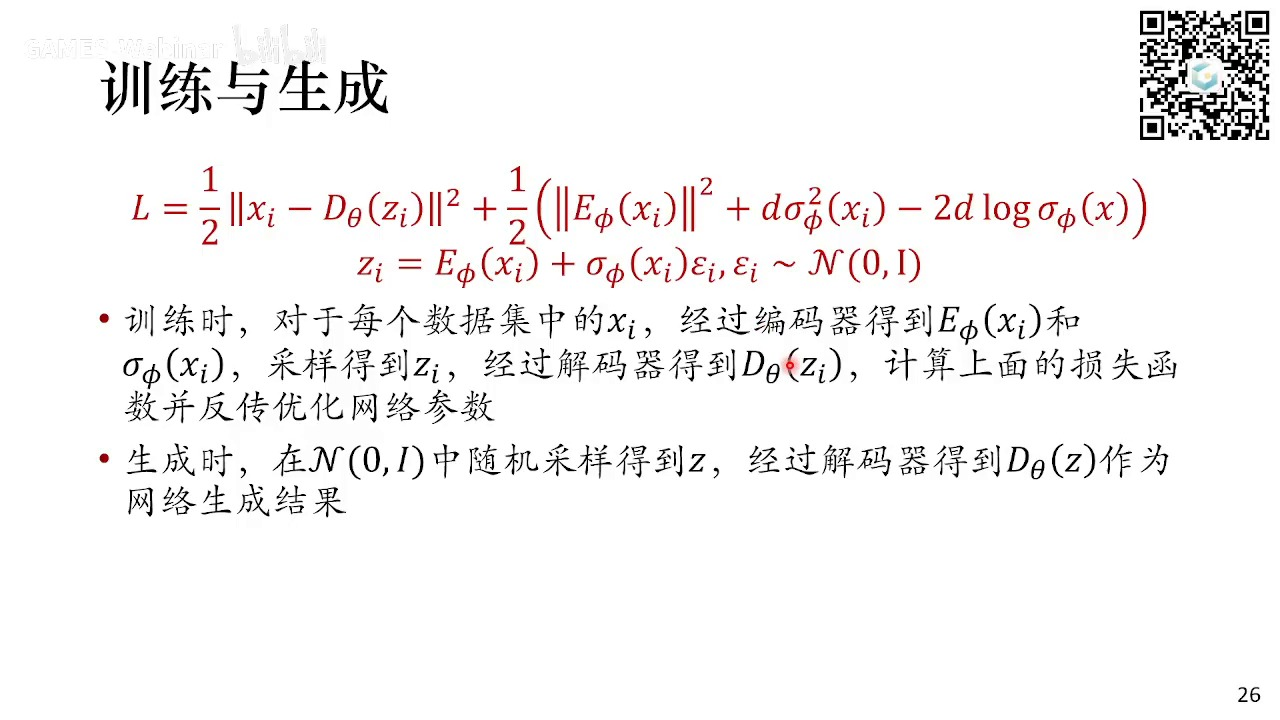
\includegraphics[width=0.92\textwidth]{figures/fig_23_vae_train.jpg}
\caption{VAE 的训练与生成\vtag}
\end{figure}
\srcnote{00:40:45--00:41:00}
\end{minipage}


把两项加起来，就是 VAE 训练时的损失函数：
\begin{equation}
L=\frac{1}{2}\|x_i-D_\theta(z_i)\|^2+\frac{1}{2}\left(\|E_\phi(x_i)\|^2+d\sigma_\phi^2(x_i)-2d\log\sigma_\phi(x_i)\right),\qquad z_i=E_\phi(x_i)+\sigma_\phi(x_i)\varepsilon_i .
\end{equation}
训练时，对于数据集中的每个 $x_i$，经过编码器得到 $E_\phi(x_i)$ 和 $\sigma_\phi(x_i)$，采样得到 $z_i$，经过解码器得到 $D_\theta(z_i)$，计算上面的损失函数，把梯度相对于 $\theta$ 和 $\phi$ 算出来，反传优化网络参数。生成时，在 $\mathcal N(0,I)$ 中随机采样得到 $z$，经过解码器得到 $D_\theta(z)$，作为网络的生成结果。

\noindent\begin{minipage}{\textwidth}
\begin{figure}[H]
\centering
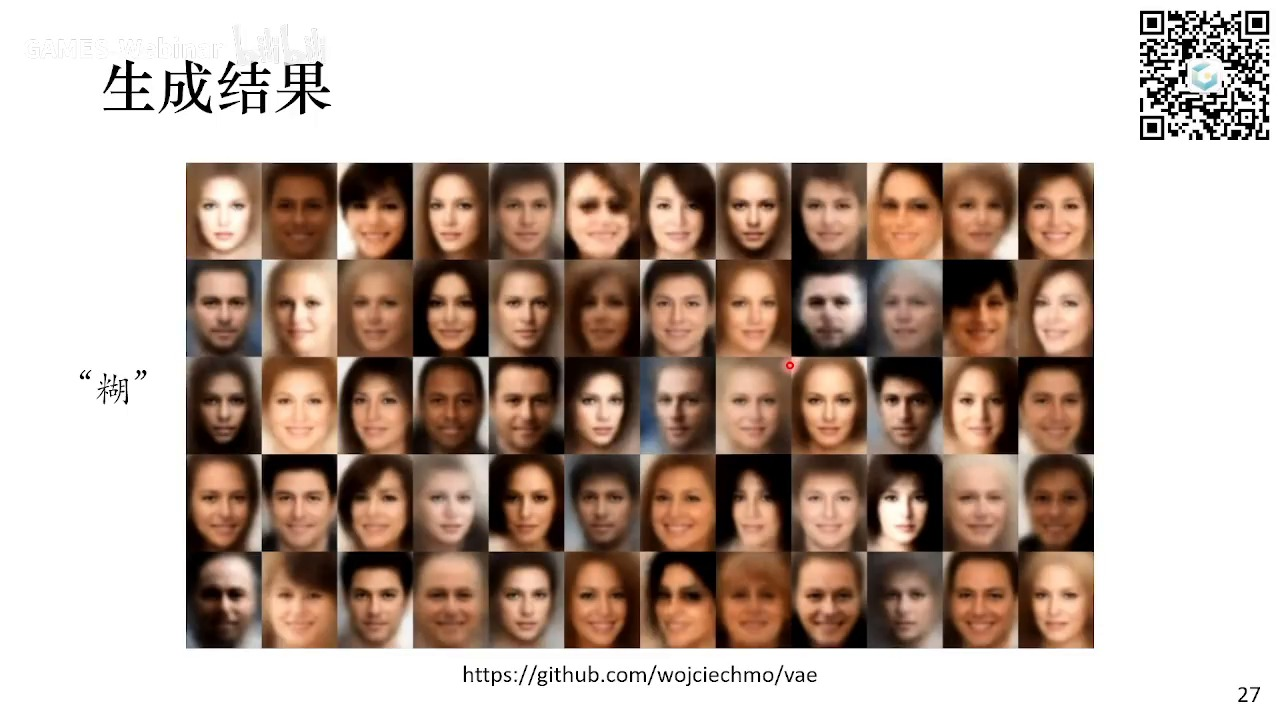
\includegraphics[width=0.92\textwidth]{figures/fig_24_vae_results.jpg}
\caption{VAE 的生成结果：“糊”\vtag}
\end{figure}
\srcnote{00:41:30--00:41:45}
\end{minipage}


课件展示了 VAE 生成的人脸，这些人脸在现实生活中并不存在。但很明显的问题是：这些人脸都非常糊。讲者解释，糊是 VAE 不得不面对的问题：中间引入了正态分布的 $z$，需要对它采样，又希望 $z$ 的方差不要太小，这就导致生成结果有些模糊。

\begin{knowledgebox}{为什么 L2 损失会“糊”}
讲义作者补充：重建项是 L2 距离，相当于假设 $p_\theta(x\mid z)$ 是方差固定的高斯分布。当同一片 $z$ 可能对应好几种合理的图像时，使 L2 误差最小的输出是这些图像的平均，而平均图像的高频细节会相互抵消，看起来就是模糊的。
\end{knowledgebox}

\section{从 VAE 理解扩散模型}

\noindent\begin{minipage}{\textwidth}
\begin{figure}[H]
\centering
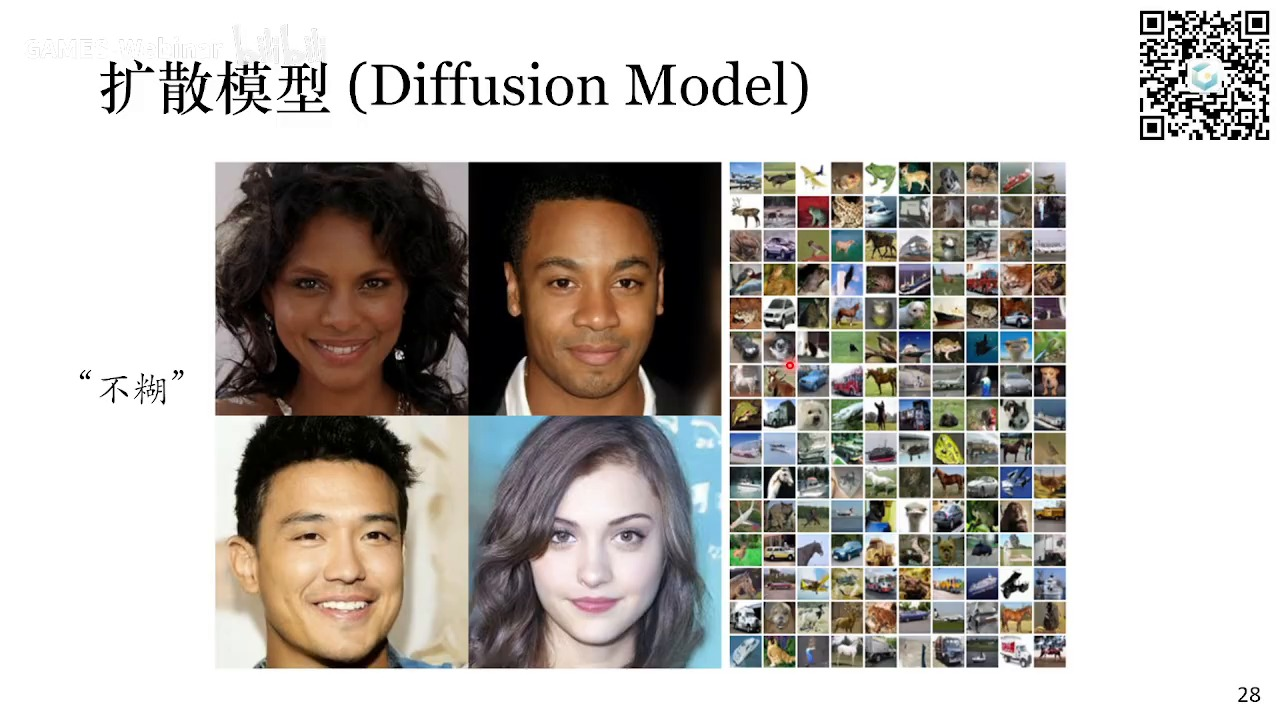
\includegraphics[width=0.92\textwidth]{figures/fig_25_diffusion_results.jpg}
\caption{扩散模型的生成结果：“不糊”\vtag}
\end{figure}
\srcnote{00:42:30--00:42:45}
\end{minipage}


与 VAE 相比，扩散模型生成的人脸不糊，讲者说如果不仔细看，甚至仔细看，都很难发现这些人脸有哪里不对，效果非常好。扩散模型可以作为一种理解方法，看成一个“高级版”的 VAE，它的很多建模和推导都与 VAE 相通。

\noindent\begin{minipage}{\textwidth}
\begin{figure}[H]
\centering
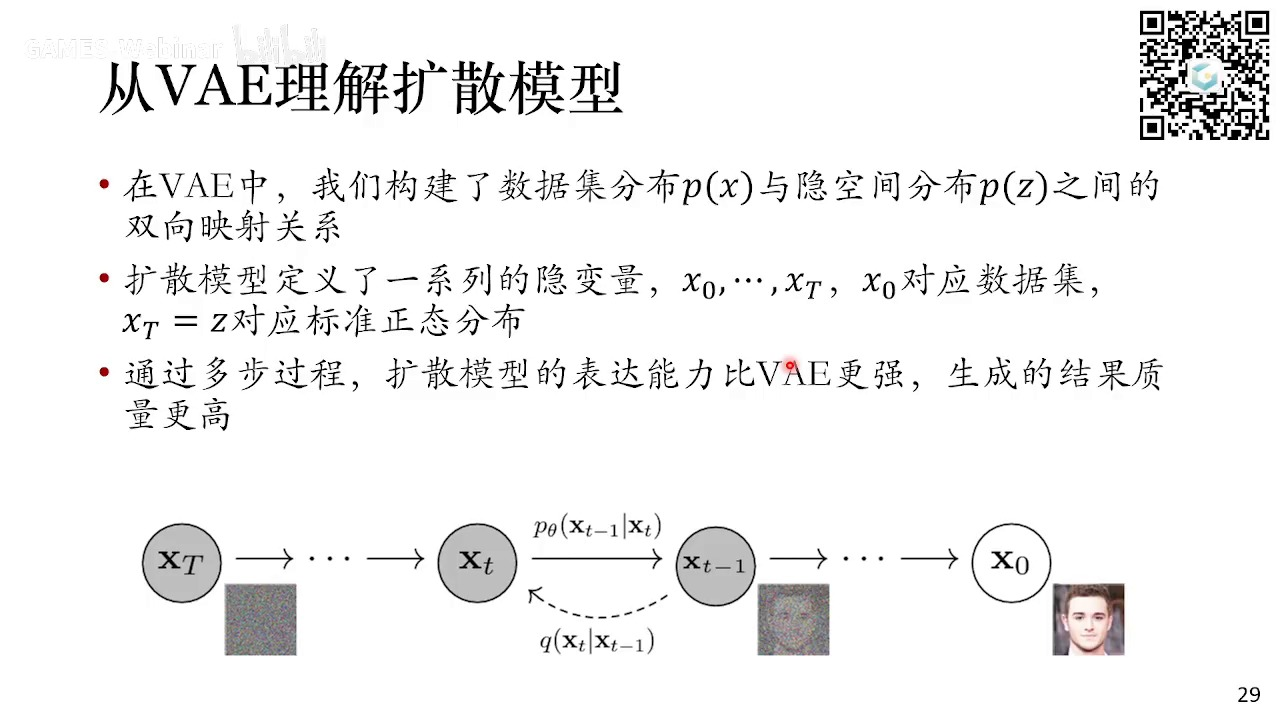
\includegraphics[width=0.92\textwidth]{figures/fig_26_vae_to_diffusion.jpg}
\caption{从 VAE 理解扩散模型：一串隐变量\vtag}
\end{figure}
\srcnote{00:44:45--00:45:00}
\end{minipage}


在 VAE 中，数据分布是未知的，隐空间分布是已知的，用编码器和解码器构建了两个方向的条件概率，即数据集分布 $p(x)$ 与隐空间分布 $p(z)$ 之间的双向映射关系。扩散模型则定义了一系列的隐变量 $x_0,\dots,x_T$：$x_0$ 对应数据集，$x_T=z$ 对应标准正态分布。通过多步过程，扩散模型的表达能力比 VAE 更强，生成的结果质量更高。

\noindent\begin{minipage}{\textwidth}
\begin{figure}[H]
\centering
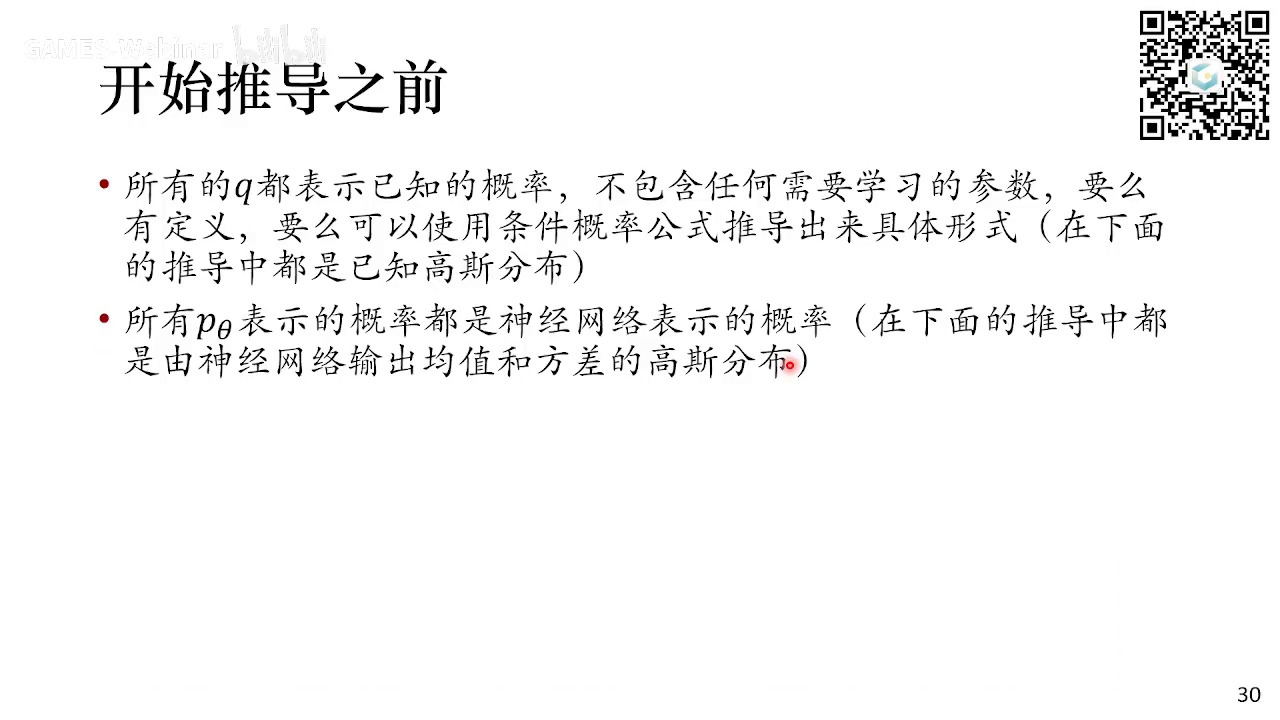
\includegraphics[width=0.92\textwidth]{figures/fig_27_notation.jpg}
\caption{开始推导之前的约定：$q$ 表示已知概率，$p_\theta$ 表示网络概率\vtag}
\end{figure}
\srcnote{00:46:15--00:46:30}
\end{minipage}


讲者提醒，扩散模型的数学非常复杂，这部分应该是整个课程中介绍的数学里最难的部分，希望大家把大的脉络搞清楚，细节可以自己去推。开始推导之前先做约定：所有的 $q$ 都表示已知的概率，不包含任何需要学习的参数，要么有定义，要么可以用条件概率公式推导出具体形式，在下面的推导中它们都是已知的高斯分布；所有 $p_\theta$ 表示的概率都是神经网络表示的概率，在下面的推导中都是由神经网络输出均值和方差的高斯分布。

\section{前向过程}

\subsection{马尔可夫链}

\noindent\begin{minipage}{\textwidth}
\begin{figure}[H]
\centering
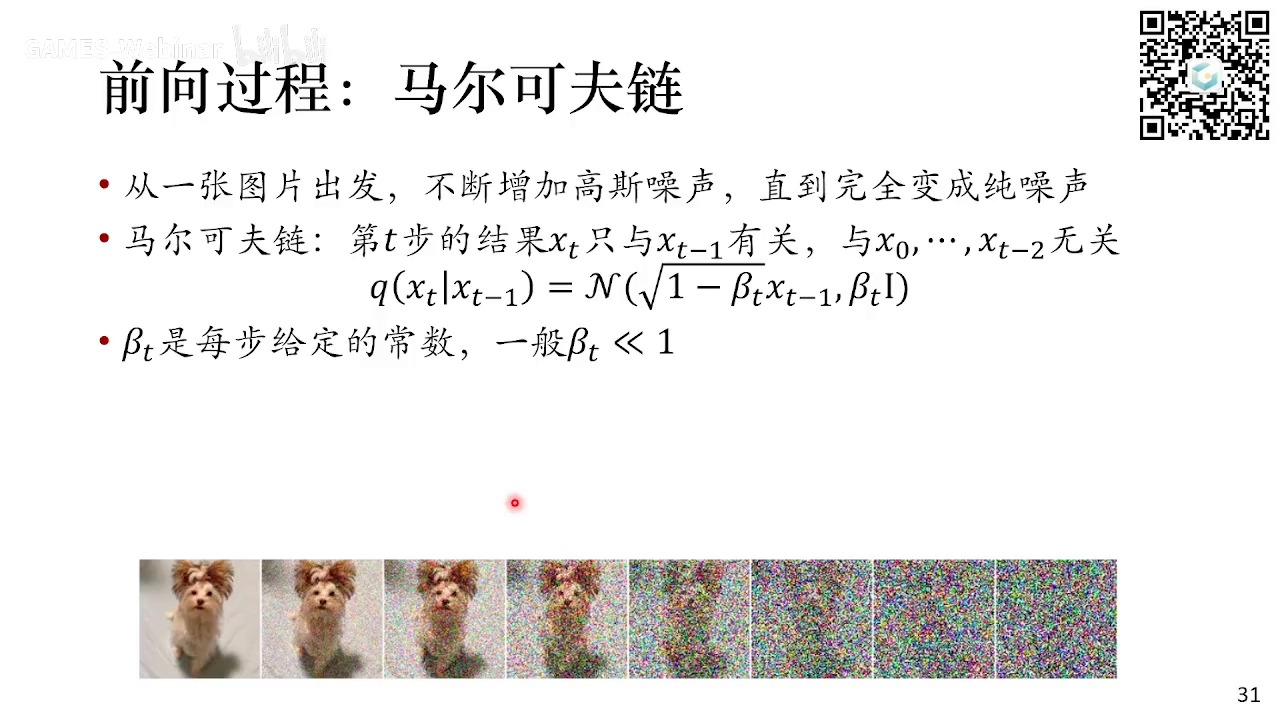
\includegraphics[width=0.92\textwidth]{figures/fig_28_forward.jpg}
\caption{前向过程：从图片出发不断增加高斯噪声\vtag}
\end{figure}
\srcnote{00:49:00--00:49:15}
\end{minipage}


前向过程从一张图片出发，不断增加高斯噪声，直到完全变成纯噪声。它是一个马尔可夫链：第 $t$ 步的结果 $x_t$ 只与 $x_{t-1}$ 有关，与 $x_0,\dots,x_{t-2}$ 无关，这叫无后效性。

\begin{knowledgebox}{马尔可夫链的无后效性}
马尔可夫链的含义是：已知当前状态后，未来与过去无关，即 $q(x_t\mid x_{t-1},\dots,x_0)=q(x_t\mid x_{t-1})$。整条链的联合分布因此可以写成单步转移的连乘 $q(x_1\cdots x_T\mid x_0)=\prod_{t=1}^{T}q(x_t\mid x_{t-1})$，后面损失函数的拆分正是基于这一点。
\end{knowledgebox}
状态转移定义为
\begin{equation}
q(x_t\mid x_{t-1})=\mathcal N\left(\sqrt{1-\beta_t}\,x_{t-1},\ \beta_tI\right),
\end{equation}
$\beta_t$ 是每步给定的常数，一般 $\beta_t\ll 1$。讲者解释：如果 $\beta_t=1$，均值的系数为零，代表完全变成噪声；$\beta_t$ 在零到一之间并且接近零，代表每一步往 $x_{t-1}$ 里加了很小的噪声。

\subsection{展开多步}

\noindent\begin{minipage}{\textwidth}
\begin{figure}[H]
\centering
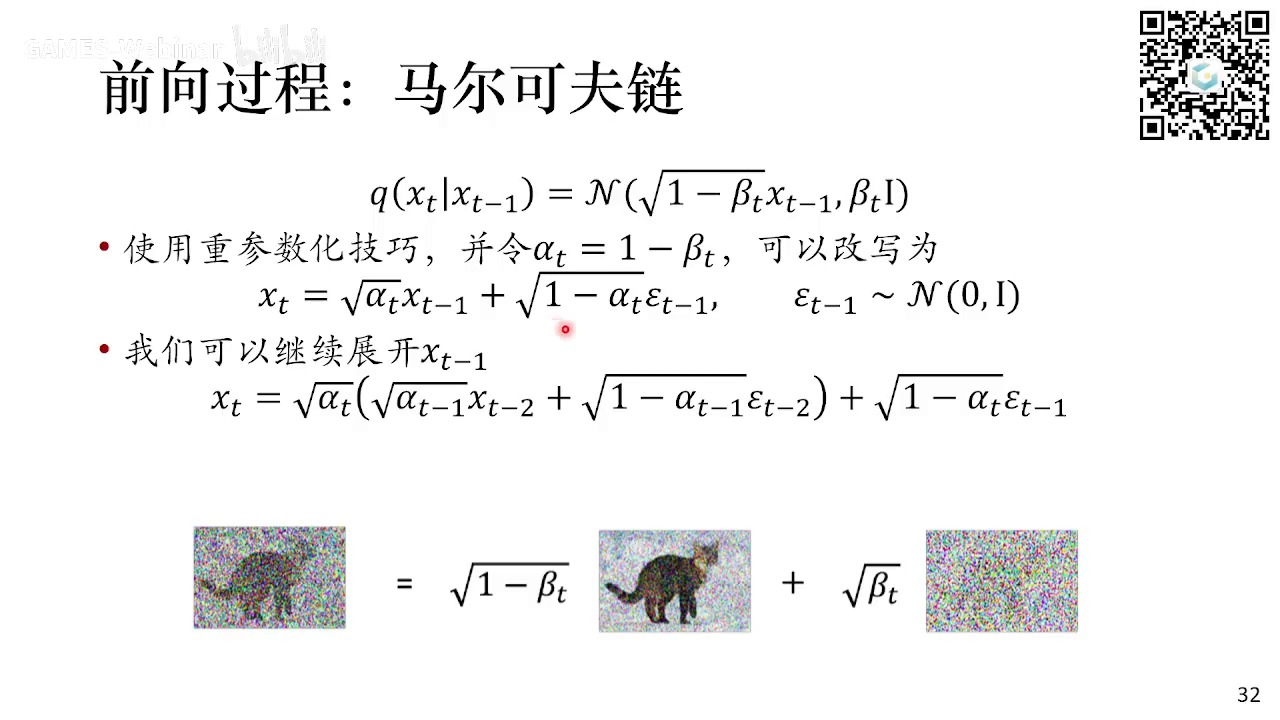
\includegraphics[width=0.92\textwidth]{figures/fig_29_forward_expand.jpg}
\caption{使用重参数化改写前向过程并继续展开\vtag}
\end{figure}
\srcnote{00:50:00--00:50:15}
\end{minipage}


使用重参数化技巧，并令 $\alpha_t=1-\beta_t$，可以改写为
\begin{equation}
x_t=\sqrt{\alpha_t}\,x_{t-1}+\sqrt{1-\alpha_t}\,\varepsilon_{t-1},\qquad \varepsilon_{t-1}\sim\mathcal N(0,I).
\end{equation}
讲者说这个写法与从高斯分布里采样是等价的，只是方便推导。继续展开 $x_{t-1}$：
\begin{equation}
x_t=\sqrt{\alpha_t}\left(\sqrt{\alpha_{t-1}}\,x_{t-2}+\sqrt{1-\alpha_{t-1}}\,\varepsilon_{t-2}\right)+\sqrt{1-\alpha_t}\,\varepsilon_{t-1}.
\end{equation}

\noindent\begin{minipage}{\textwidth}
\begin{figure}[H]
\centering
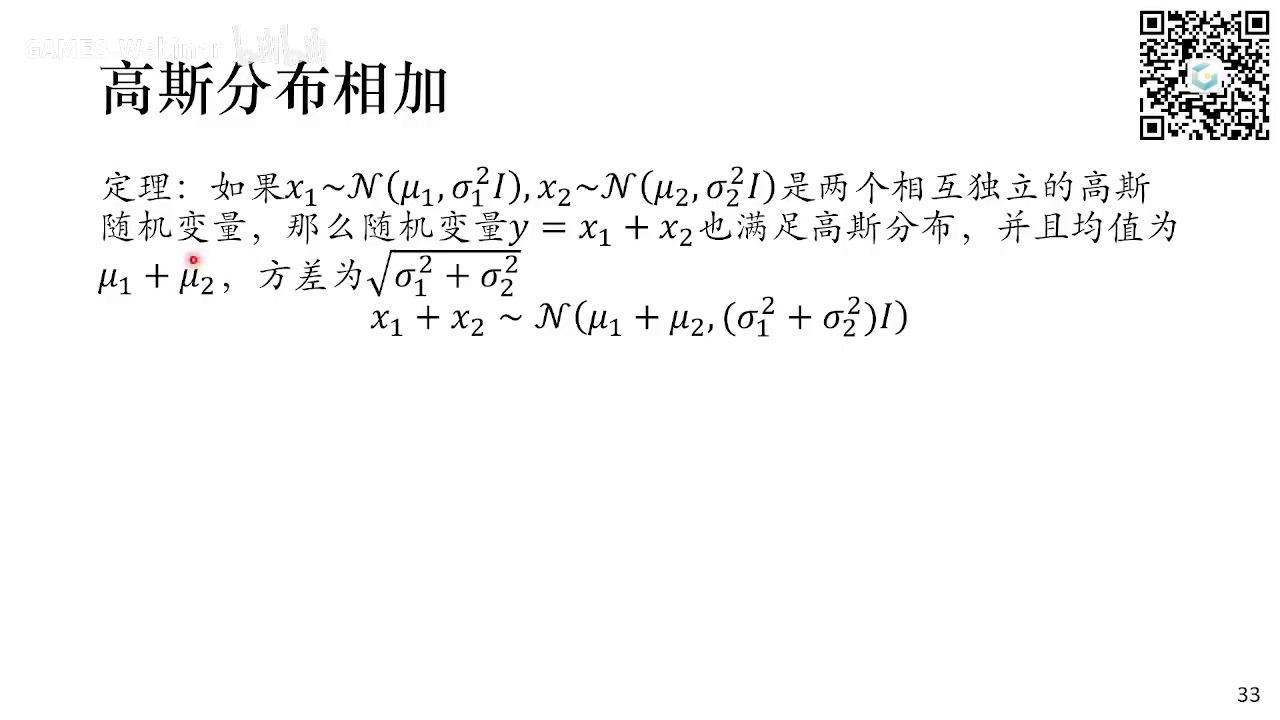
\includegraphics[width=0.92\textwidth]{figures/fig_30_gauss_sum.jpg}
\caption{高斯分布相加定理\vtag}
\end{figure}
\srcnote{00:50:45--00:51:00}
\end{minipage}


这里需要一个定理：如果 $x_1\sim\mathcal N(\mu_1,\sigma_1^2I)$ 和 $x_2\sim\mathcal N(\mu_2,\sigma_2^2I)$ 是两个相互独立的高斯随机变量，那么 $y=x_1+x_2$ 也服从高斯分布，均值为 $\mu_1+\mu_2$，方差为 $\sigma_1^2+\sigma_2^2$：
\begin{equation}
x_1+x_2\sim\mathcal N\left(\mu_1+\mu_2,\ (\sigma_1^2+\sigma_2^2)I\right).
\end{equation}

\noindent\begin{minipage}{\textwidth}
\begin{figure}[H]
\centering
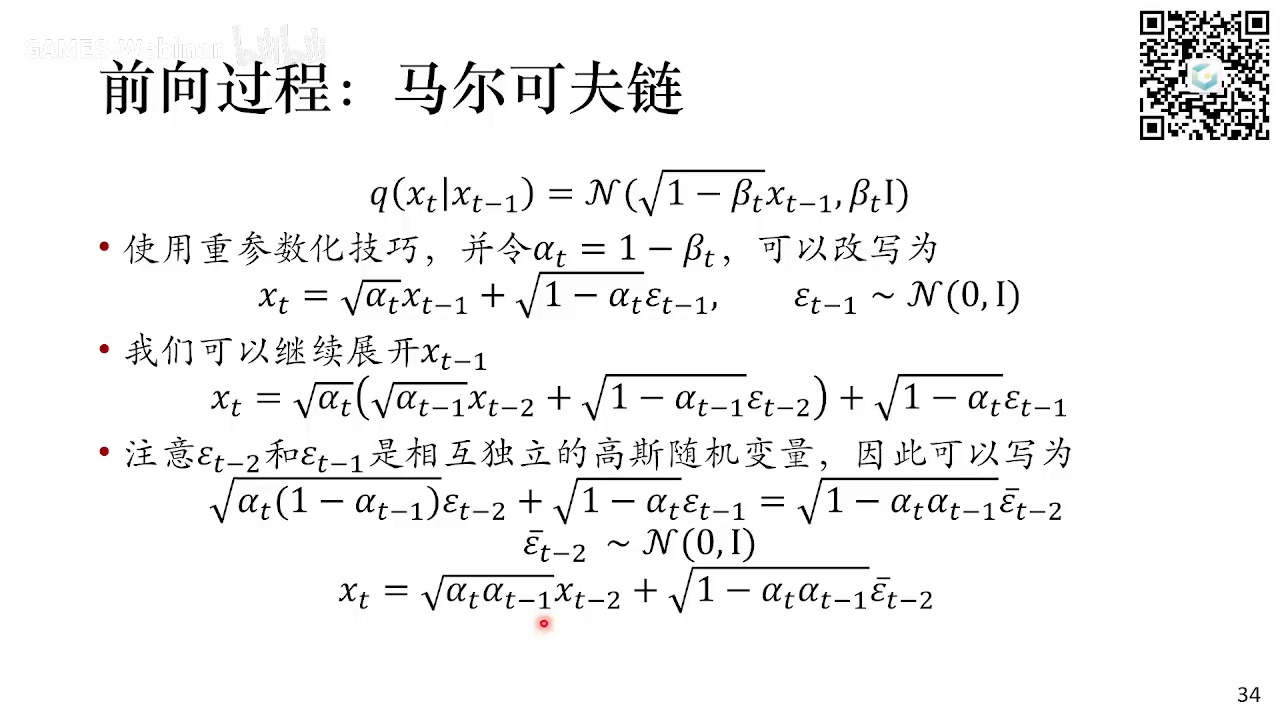
\includegraphics[width=0.92\textwidth]{figures/fig_31_forward_merge.jpg}
\caption{两步加噪可以合并为一步加更大的噪声\vtag}
\end{figure}
\srcnote{00:51:45--00:52:00}
\end{minipage}


注意 $\varepsilon_{t-2}$ 和 $\varepsilon_{t-1}$ 是相互独立的高斯随机变量，两个噪声项的方差分别为 $\alpha_t(1-\alpha_{t-1})$ 和 $1-\alpha_t$，加起来是 $1-\alpha_t\alpha_{t-1}$。因此可以合并为
\begin{equation}
\sqrt{\alpha_t(1-\alpha_{t-1})}\,\varepsilon_{t-2}+\sqrt{1-\alpha_t}\,\varepsilon_{t-1}=\sqrt{1-\alpha_t\alpha_{t-1}}\,\bar\varepsilon_{t-2},\qquad \bar\varepsilon_{t-2}\sim\mathcal N(0,I),
\end{equation}
即 $x_t=\sqrt{\alpha_t\alpha_{t-1}}\,x_{t-2}+\sqrt{1-\alpha_t\alpha_{t-1}}\,\bar\varepsilon_{t-2}$。

\subsection{一步得到任意时刻}

\noindent\begin{minipage}{\textwidth}
\begin{figure}[H]
\centering
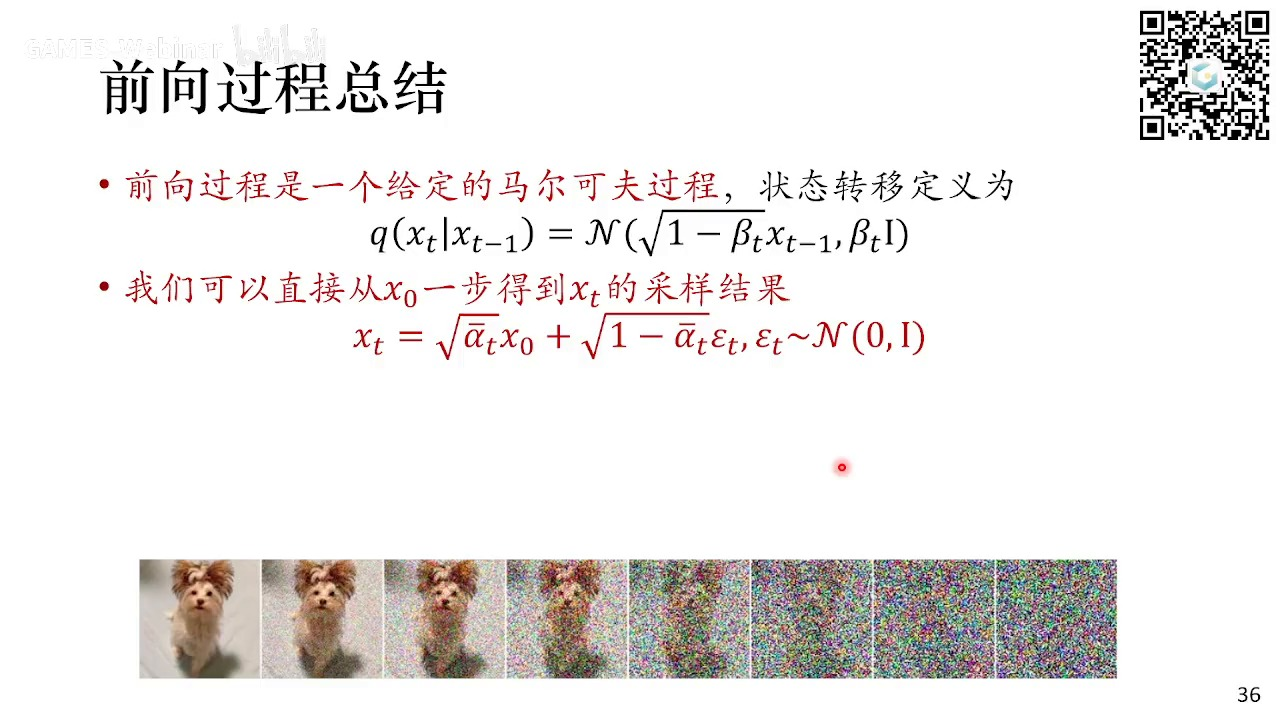
\includegraphics[width=0.92\textwidth]{figures/fig_32_forward_summary.jpg}
\caption{前向过程总结：可以从 $x_0$ 一步得到 $x_t$\vtag}
\end{figure}
\srcnote{00:53:00--00:53:15}
\end{minipage}


比较 $x_t$ 关于 $x_{t-1}$ 和关于 $x_{t-2}$ 的两个式子，形式非常相似，意味着两步加噪的过程可以看成一步加了更大的噪声。这个展开过程可以持续下去，得到 $x_t$ 与真实图片 $x_0$ 之间的关系，其中 $\bar\alpha_t=\alpha_t\alpha_{t-1}\cdots\alpha_1$：
\begin{equation}
x_t=\sqrt{\bar\alpha_t}\,x_0+\sqrt{1-\bar\alpha_t}\,\varepsilon_t,\qquad \varepsilon_t\sim\mathcal N(0,I).
\end{equation}
讲者强调，这是扩散模型前向过程中最重要的结论，对后面的推导非常有用：前向过程是一个给定的马尔可夫过程，但我们可以直接从 $x_0$ 一步得到 $x_t$ 的采样结果。

\begin{practicebox}{检验前向过程的终点}
讲义作者补充：读者可以验证 $x_t$ 的方差为 $\bar\alpha_t\operatorname{Var}(x_0)+(1-\bar\alpha_t)$。若数据已归一化到单位方差，则每一步方差都保持为一，这正是均值系数取 $\sqrt{1-\beta_t}$ 而不是 $1$ 的原因。由于每个 $\alpha_t<1$，当 $T$ 足够大时 $\bar\alpha_T\to 0$，$x_T$ 就近似为标准正态，与 $x_0$ 无关。
\end{practicebox}

\section{反向过程与损失函数}

\subsection{反向过程}

\noindent\begin{minipage}{\textwidth}
\begin{figure}[H]
\centering
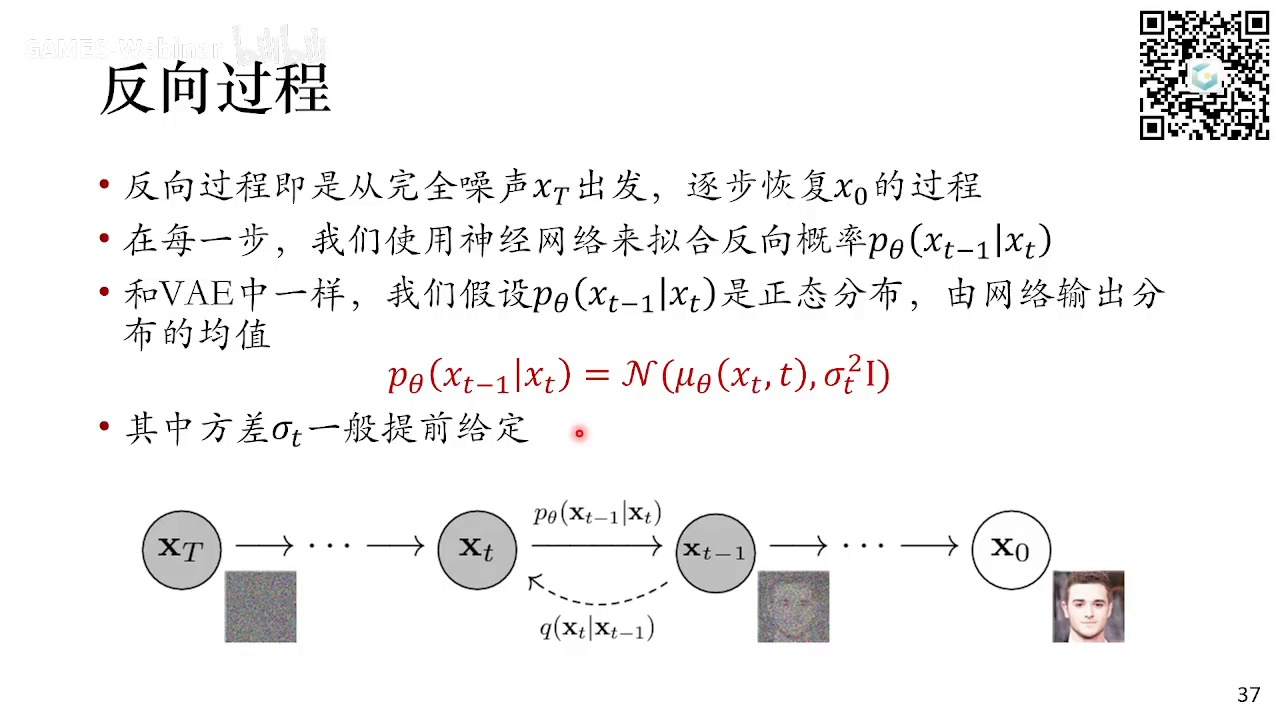
\includegraphics[width=0.92\textwidth]{figures/fig_33_reverse.jpg}
\caption{反向过程：用神经网络拟合每一步的反向概率\vtag}
\end{figure}
\srcnote{00:54:00--00:54:15}
\end{minipage}


反向过程是从完全噪声 $x_T$ 出发，逐步恢复 $x_0$ 的过程。在每一步，使用神经网络来拟合反向概率 $p_\theta(x_{t-1}\mid x_t)$。和 VAE 中一样，假设它是正态分布，由网络输出均值：
\begin{equation}
p_\theta(x_{t-1}\mid x_t)=\mathcal N\left(\mu_\theta(x_t,t),\ \sigma_t^2I\right),
\end{equation}
方差 $\sigma_t$ 一般提前给定，可以取一个较小的值。

\subsection{与 VAE 相同的目标}

\noindent\begin{minipage}{\textwidth}
\begin{figure}[H]
\centering
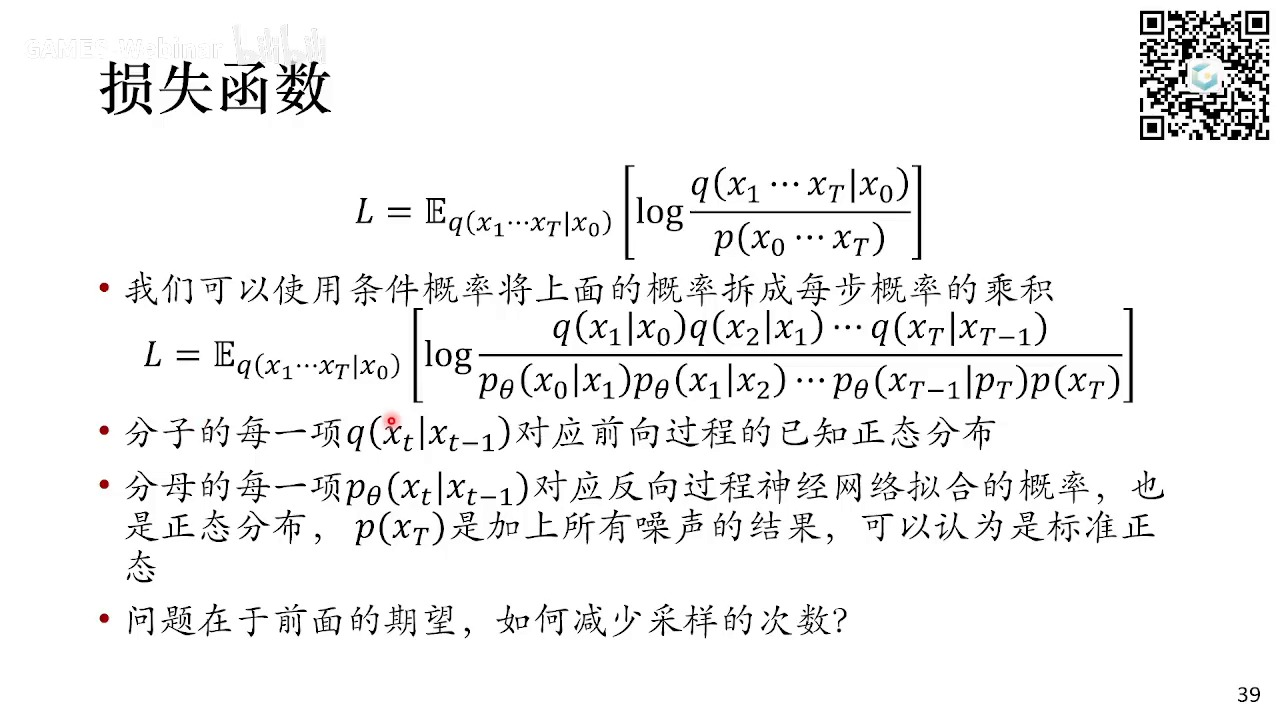
\includegraphics[width=0.92\textwidth]{figures/fig_34_diff_loss1.jpg}
\caption{扩散模型的损失函数：与 VAE 相同的 ELBO 目标\vtag}
\end{figure}
\srcnote{00:57:00--00:57:15}
\end{minipage}


对于 VAE，优化的是 ELBO 损失函数 $L=\mathbb E_{z\sim q_\phi(z\mid x)}\log\frac{q_\phi(z\mid x)}{p(x,z)}$。对于扩散模型，优化相同的目标，只不过现在隐变量包含 $x_T,\dots,x_1$，而数据集采样对应 $x_0$。只需做变量替换，扩散模型的损失函数可以定义为
\begin{equation}
L=\mathbb E_{q(x_1\cdots x_T\mid x_0)}\log\frac{q(x_1\cdots x_T\mid x_0)}{p(x_0\cdots x_T)} .
\end{equation}
用条件概率把它拆成每步概率的乘积：
\begin{equation}
L=\mathbb E_{q(x_1\cdots x_T\mid x_0)}\log\frac{q(x_1\mid x_0)q(x_2\mid x_1)\cdots q(x_T\mid x_{T-1})}{p_\theta(x_0\mid x_1)p_\theta(x_1\mid x_2)\cdots p_\theta(x_{T-1}\mid x_T)p(x_T)} .
\end{equation}
分子的每一项 $q(x_t\mid x_{t-1})$ 对应前向过程的已知正态分布；分母的每一项对应反向过程神经网络拟合的概率，也是正态分布，$p(x_T)$ 是加上所有噪声的结果，可以认为是标准正态。问题在于前面的期望：采样空间非常非常大，直接采样显然不可能，如何减少采样次数？

\subsection{引入 $x_0$ 作为条件}

\noindent\begin{minipage}{\textwidth}
\begin{figure}[H]
\centering
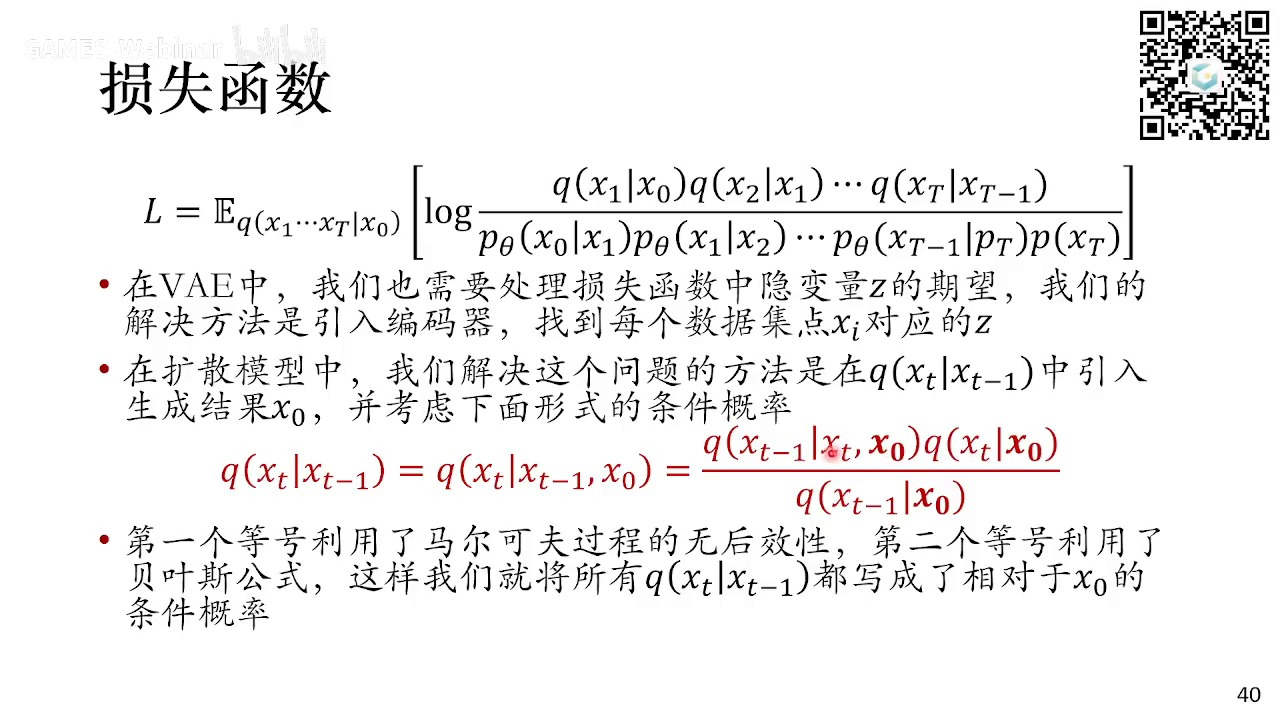
\includegraphics[width=0.92\textwidth]{figures/fig_35_diff_loss2.jpg}
\caption{在前向转移中引入 $x_0$，用贝叶斯公式改写\vtag}
\end{figure}
\srcnote{00:59:30--00:59:45}
\end{minipage}


回顾 VAE 的做法：引入编码器，找到每个数据点 $x_i$ 对应的 $z$。在扩散模型中，解决方法是在 $q(x_t\mid x_{t-1})$ 中引入 $x_0$，考虑下面形式的条件概率：
\begin{equation}
q(x_t\mid x_{t-1})=q(x_t\mid x_{t-1},x_0)=\frac{q(x_{t-1}\mid x_t,x_0)\,q(x_t\mid x_0)}{q(x_{t-1}\mid x_0)} .
\end{equation}
第一个等号利用了马尔可夫过程的无后效性，$x_t$ 只依赖 $x_{t-1}$，额外加上条件 $x_0$ 不改变它；第二个等号利用了贝叶斯公式。

\noindent\begin{minipage}{\textwidth}
\begin{figure}[H]
\centering
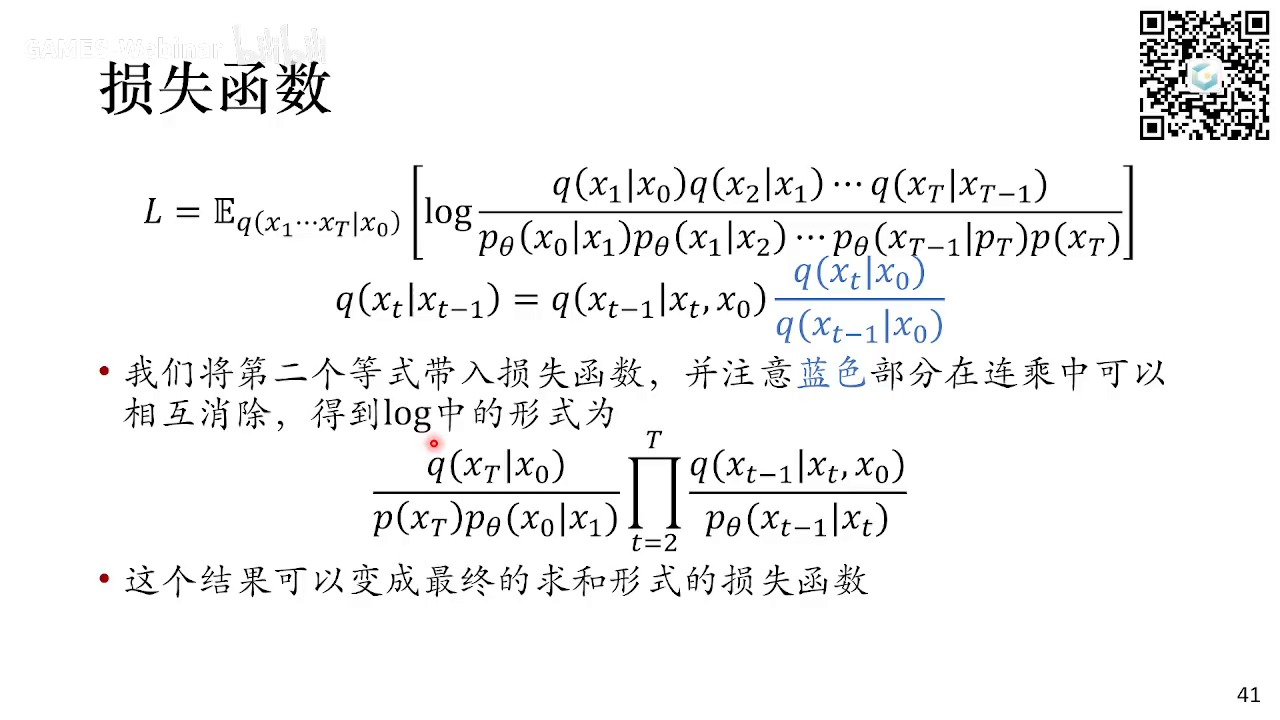
\includegraphics[width=0.92\textwidth]{figures/fig_36_diff_loss3.jpg}
\caption{代入后连乘中相邻项相互消去\vtag}
\end{figure}
\srcnote{01:00:30--01:00:45}
\end{minipage}


把它代入损失函数，形如 $q(x_t\mid x_0)/q(x_{t-1}\mid x_0)$ 的部分在连乘中相邻项相互消去，得到对数里的形式为
\begin{equation}
\frac{q(x_T\mid x_0)}{p(x_T)\,p_\theta(x_0\mid x_1)}\prod_{t=2}^{T}\frac{q(x_{t-1}\mid x_t,x_0)}{p_\theta(x_{t-1}\mid x_t)} .
\end{equation}

\subsection{三项损失}

\noindent\begin{minipage}{\textwidth}
\begin{figure}[H]
\centering
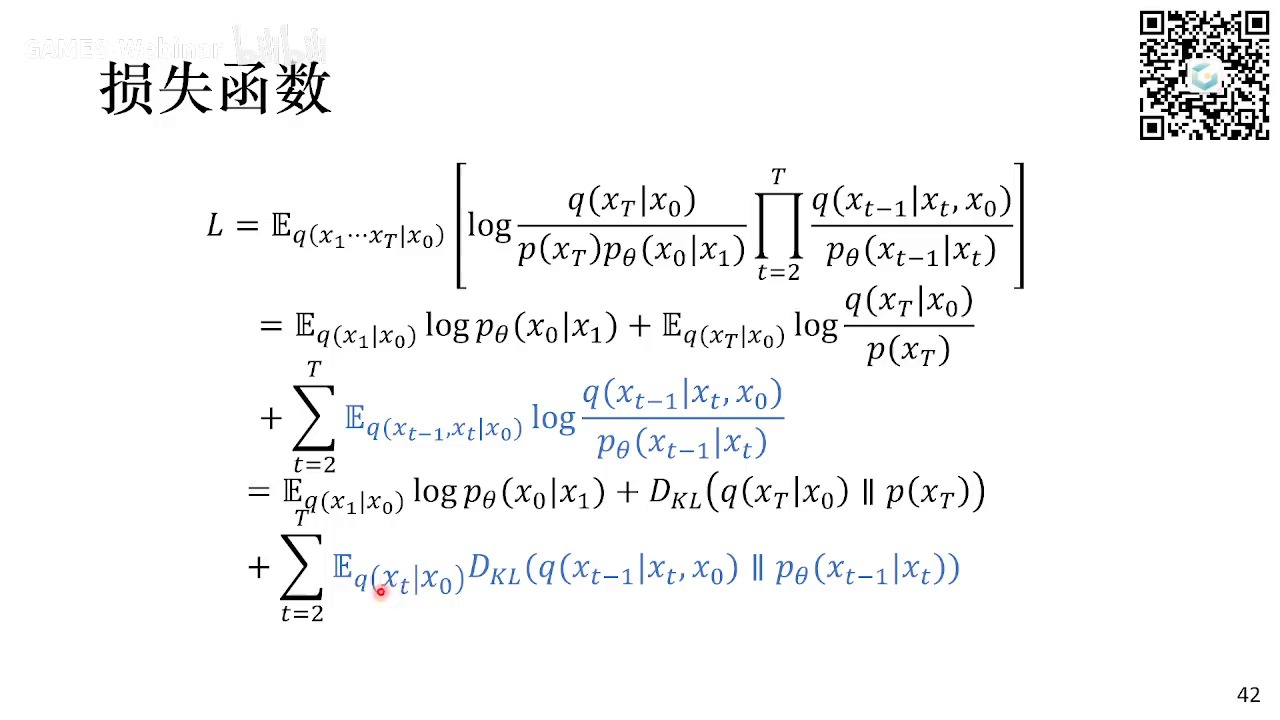
\includegraphics[width=0.92\textwidth]{figures/fig_37_diff_loss4.jpg}
\caption{损失函数整理为三项\vtag}
\end{figure}
\srcnote{01:02:45--01:03:00}
\end{minipage}


对数把连乘变成求和。每一项只与少数几个变量有关，例如第一项只与 $x_0,x_1$ 有关，前面对其他变量的采样求均值就根本不需要做。整理后得到
\begin{equation}
\begin{aligned}
L&=\mathbb E_{q(x_1\mid x_0)}\left[-\log p_\theta(x_0\mid x_1)\right]+D_{\mathrm{KL}}\big(q(x_T\mid x_0)\,\|\,p(x_T)\big)\\
&\quad+\sum_{t=2}^{T}\mathbb E_{q(x_t\mid x_0)}D_{\mathrm{KL}}\big(q(x_{t-1}\mid x_t,x_0)\,\|\,p_\theta(x_{t-1}\mid x_t)\big).
\end{aligned}
\end{equation}

\begin{warningbox}{第一项的符号}
课件上第一项写作 $\mathbb E_{q(x_1\mid x_0)}\log p_\theta(x_0\mid x_1)$。讲义作者按推导核对：对数里的因子是 $1/p_\theta(x_0\mid x_1)$，所以这一项应带负号，即 $-\log p_\theta(x_0\mid x_1)$，与 VAE 中的重建项 $-\log p_\theta(x_i\mid z)$ 对应。最小化损失时它要求网络把 $x_1$ 还原成 $x_0$ 的概率尽可能大。
\end{warningbox}

\noindent\begin{minipage}{\textwidth}
\begin{figure}[H]
\centering
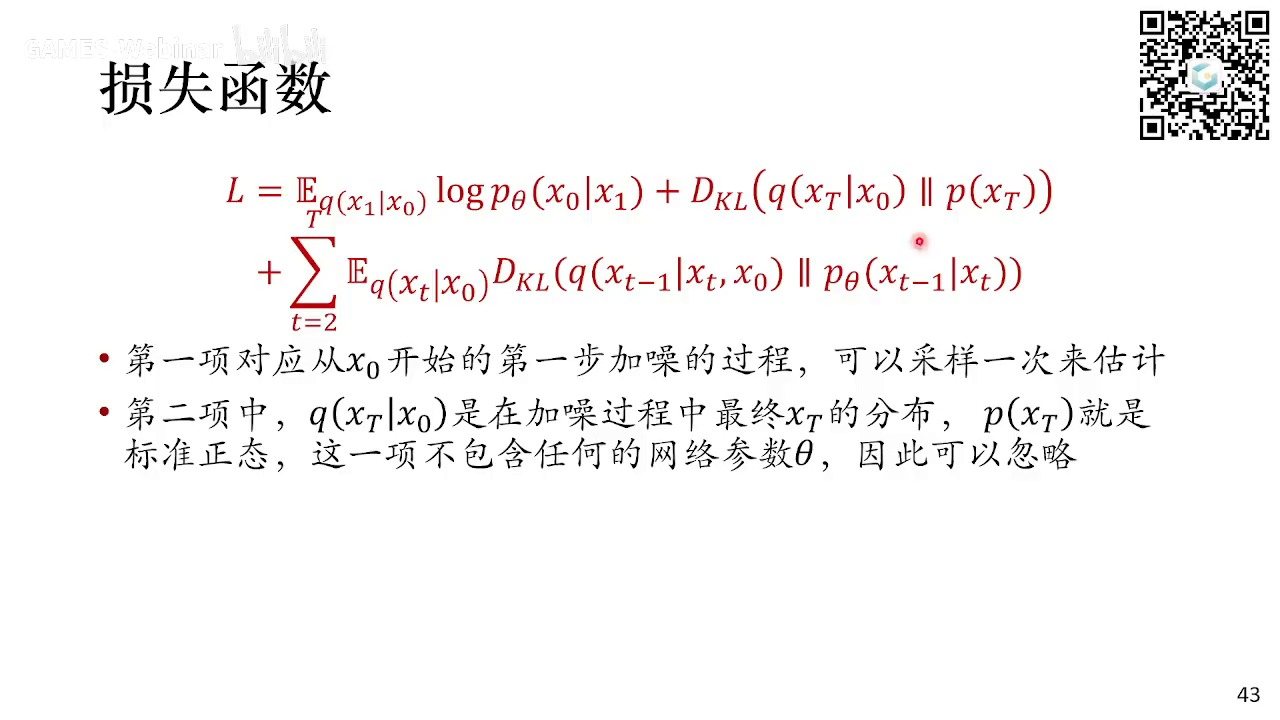
\includegraphics[width=0.92\textwidth]{figures/fig_38_diff_terms.jpg}
\caption{逐项分析：第一项采样一次，第二项与网络无关\vtag}
\end{figure}
\srcnote{01:04:30--01:04:45}
\end{minipage}


讲者一项一项地看：第一项对应从 $x_0$ 开始第一步加噪的过程，加的是方差很小的噪声，采样一次就足以估计均值；第二项中，$q(x_T\mid x_0)$ 是加噪过程中最终 $x_T$ 的分布，$p(x_T)$ 就是标准正态，这一项不包含任何网络参数 $\theta$，因此可以忽略；剩下的就是反向过程中每一步的损失函数，可以理解为希望网络概率 $p_\theta(x_{t-1}\mid x_t)$ 与 $q(x_{t-1}\mid x_t,x_0)$ 尽可能接近：
\begin{equation}
L_t=\mathbb E_{q(x_t\mid x_0)}D_{\mathrm{KL}}\big(q(x_{t-1}\mid x_t,x_0)\,\|\,p_\theta(x_{t-1}\mid x_t)\big).
\end{equation}
由于前向过程可以由 $x_0$ 直接得到 $x_t$，不需要跑完整个前向过程，实际训练时会把 $L$ 中的求和改成对 $t$ 的期望：对数据集中的每张图片，只均匀随机采样一个 $t$，用这一项 $L_t$ 作为损失。

\subsection{后验分布的具体形式}

\noindent\begin{minipage}{\textwidth}
\begin{figure}[H]
\centering
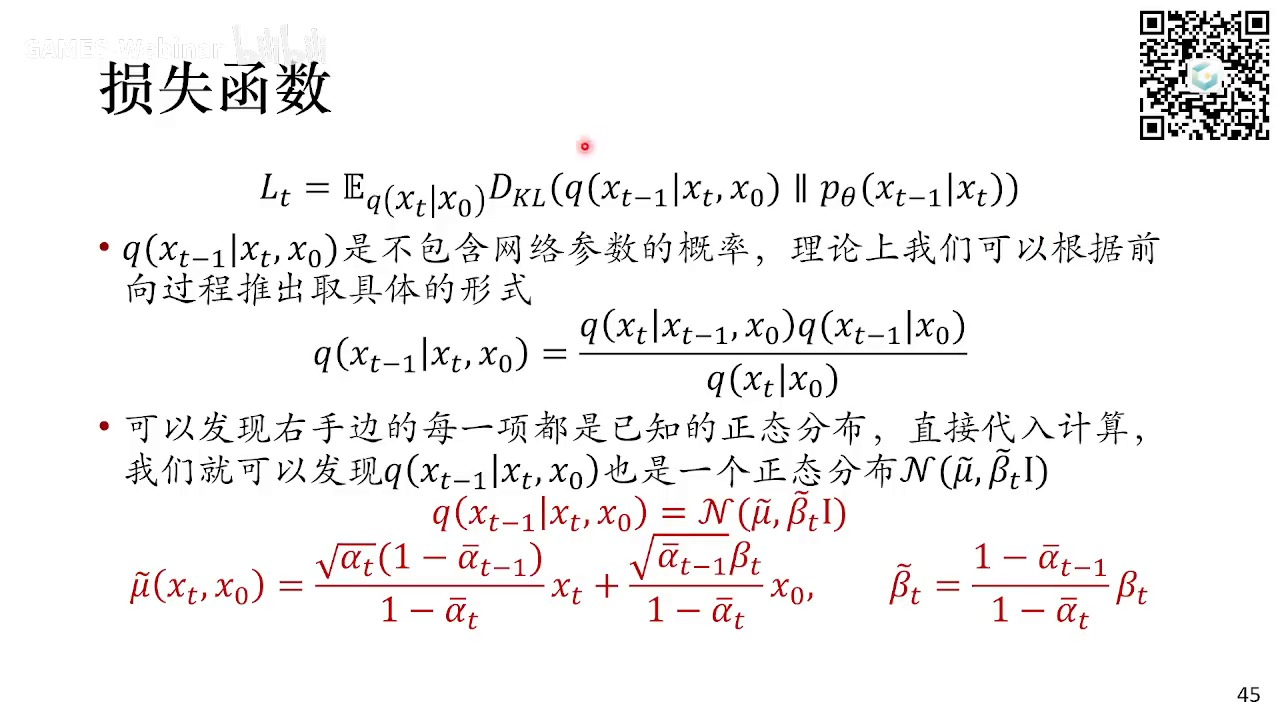
\includegraphics[width=0.92\textwidth]{figures/fig_39_posterior.jpg}
\caption{$q(x_{t-1}\mid x_t,x_0)$ 是已知的正态分布\vtag}
\end{figure}
\srcnote{01:09:15--01:09:30}
\end{minipage}


$q(x_{t-1}\mid x_t,x_0)$ 是不包含网络参数的概率，理论上可以根据前向过程推出具体形式：
\begin{equation}
q(x_{t-1}\mid x_t,x_0)=\frac{q(x_t\mid x_{t-1},x_0)\,q(x_{t-1}\mid x_0)}{q(x_t\mid x_0)} .
\end{equation}
右边每一项都是已知的正态分布：分子第一项是单步加噪的转移，第二项是加了 $t-1$ 步噪声后的分布，分母是加了 $t$ 步噪声后的分布。直接代入计算可以发现它也是一个正态分布 $\mathcal N(\tilde\mu,\tilde\beta_tI)$：
\begin{equation}
\tilde\mu(x_t,x_0)=\frac{\sqrt{\alpha_t}(1-\bar\alpha_{t-1})}{1-\bar\alpha_t}x_t+\frac{\sqrt{\bar\alpha_{t-1}}\,\beta_t}{1-\bar\alpha_t}x_0,\qquad \tilde\beta_t=\frac{1-\bar\alpha_{t-1}}{1-\bar\alpha_t}\beta_t .
\end{equation}

\subsection{化为均值之差}

\noindent\begin{minipage}{\textwidth}
\begin{figure}[H]
\centering
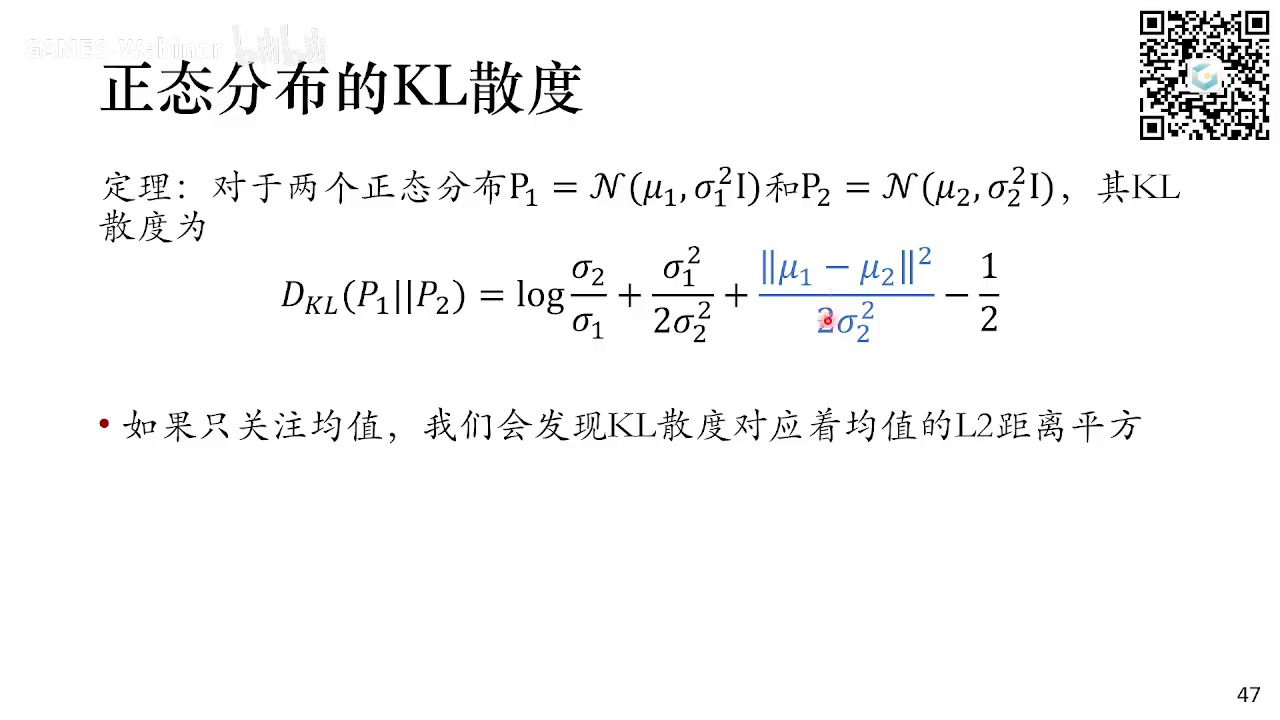
\includegraphics[width=0.92\textwidth]{figures/fig_40_diff_kl.jpg}
\caption{两个正态分布的 KL 散度只关注均值时对应 L2 距离\vtag}
\end{figure}
\srcnote{01:10:00--01:10:15}
\end{minipage}


现在 $q(x_{t-1}\mid x_t,x_0)$ 是已知的正态分布，$p_\theta(x_{t-1}\mid x_t)=\mathcal N(\mu_\theta(x_t,t),\sigma_t^2I)$ 是网络输出的正态分布，二者的 KL 散度有解析表达式。回到前面两个正态分布的 KL 散度公式：方差都是给定的，如果只关注均值，KL 散度就对应着均值的 L2 距离平方。所以在简化的情形下，可以把 KL 散度近似为两个分布均值的 L2 差距：
\begin{equation}
L_t\approx\mathbb E_{q(x_t\mid x_0)}\left\|\tilde\mu(x_t,x_0)-\mu_\theta(x_t,t)\right\|^2 .
\end{equation}
对 $q(x_t\mid x_0)$ 求期望，可以利用前向过程的关系直接对 $x_t$ 采样：$x_t=\sqrt{\bar\alpha_t}x_0+\sqrt{1-\bar\alpha_t}\varepsilon_t$。到这里已经可以计算损失函数并回传梯度了，不过扩散模型算法的最终形式还进行了一次参数变换。

\subsection{参数变换：预测噪声}

\noindent\begin{minipage}{\textwidth}
\begin{figure}[H]
\centering
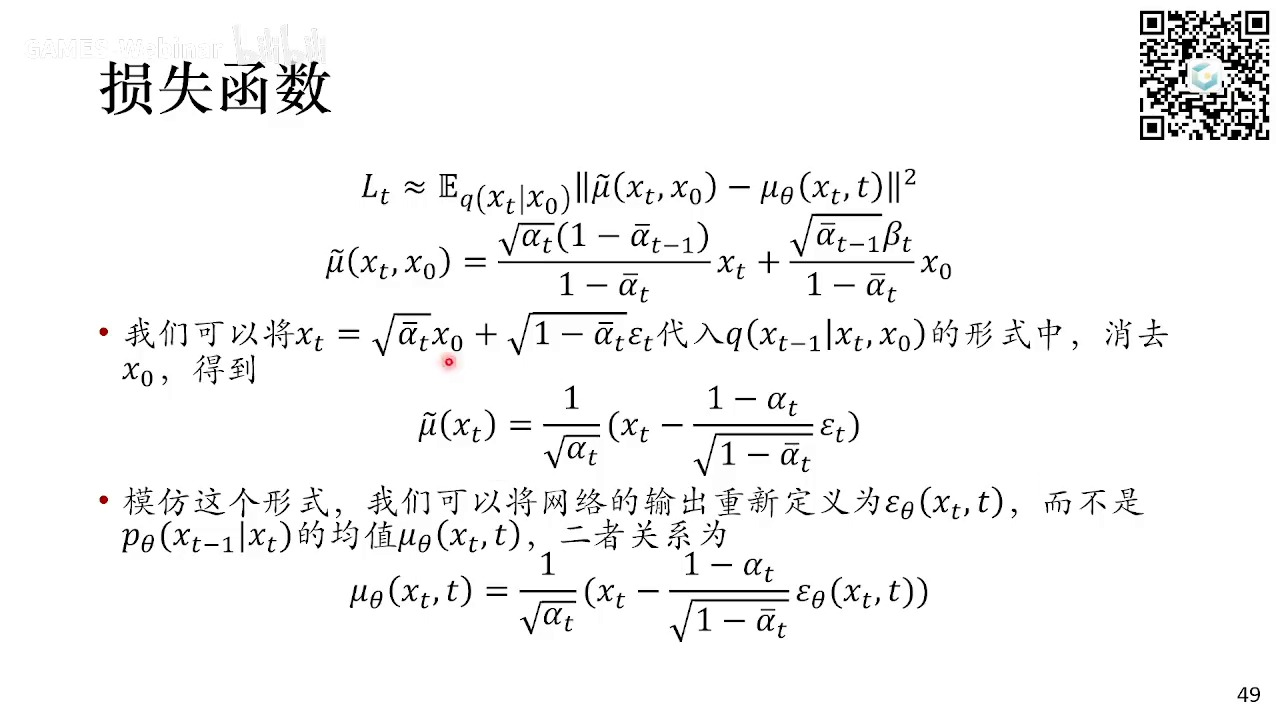
\includegraphics[width=0.92\textwidth]{figures/fig_41_eps_param.jpg}
\caption{把网络输出重新定义为噪声 $\varepsilon_\theta(x_t,t)$\vtag}
\end{figure}
\srcnote{01:13:45--01:14:00}
\end{minipage}


将 $x_t=\sqrt{\bar\alpha_t}x_0+\sqrt{1-\bar\alpha_t}\varepsilon_t$ 代入 $\tilde\mu$ 的表达式，消去 $x_0$，得到
\begin{equation}
\tilde\mu(x_t)=\frac{1}{\sqrt{\alpha_t}}\left(x_t-\frac{1-\alpha_t}{\sqrt{1-\bar\alpha_t}}\varepsilon_t\right).
\end{equation}
讲者指出，括号里这一部分对应的是纯高斯噪声。模仿这个形式，把网络的输出重新定义为噪声 $\varepsilon_\theta(x_t,t)$，而不是 $p_\theta(x_{t-1}\mid x_t)$ 的均值 $\mu_\theta(x_t,t)$，二者关系为
\begin{equation}
\mu_\theta(x_t,t)=\frac{1}{\sqrt{\alpha_t}}\left(x_t-\frac{1-\alpha_t}{\sqrt{1-\bar\alpha_t}}\varepsilon_\theta(x_t,t)\right).
\end{equation}

\noindent\begin{minipage}{\textwidth}
\begin{figure}[H]
\centering
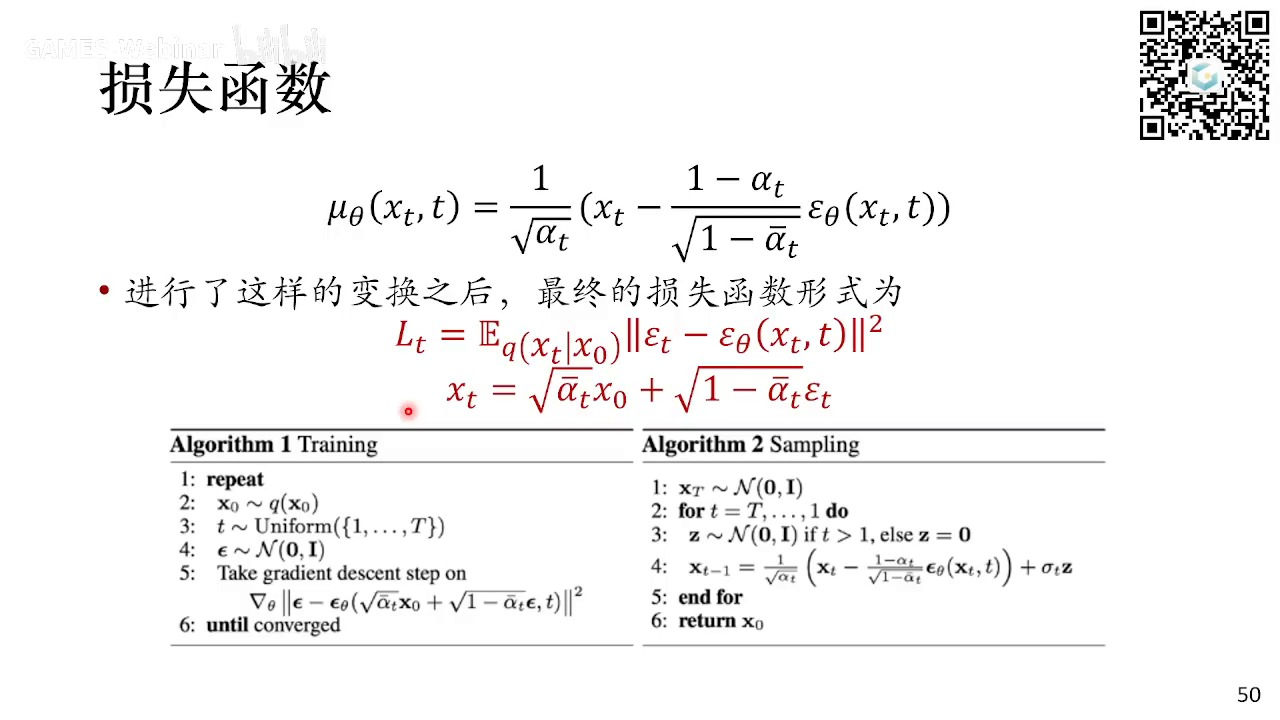
\includegraphics[width=0.92\textwidth]{figures/fig_42_final_loss.jpg}
\caption{最终的损失函数与训练、采样算法\vtag}
\end{figure}
\srcnote{01:14:30--01:14:45}
\end{minipage}


经过这样的变换，两个均值之差只剩下两个噪声之差（再乘上一个与 $\theta$ 无关的系数），最终的损失函数形式为
\begin{equation}
L_t=\mathbb E_{q(x_t\mid x_0)}\left\|\varepsilon_t-\varepsilon_\theta(x_t,t)\right\|^2,\qquad x_t=\sqrt{\bar\alpha_t}\,x_0+\sqrt{1-\bar\alpha_t}\,\varepsilon_t .
\end{equation}
其中 $\varepsilon_t$ 是纯粹的高斯噪声，是我们自己撒进去的；$\varepsilon_\theta$ 是网络预测的噪声。

\begin{importantbox}{扩散模型的训练与生成}
训练：从数据集取一张图 $x_0$，均匀随机取一个 $t$，采样噪声 $\varepsilon_t$，按前向公式一步得到 $x_t$，让网络从 $(x_t,t)$ 预测出 $\varepsilon_t$，用两者的 L2 距离平方求梯度，放进随机梯度下降中收敛。生成：从完全随机的噪声 $x_T$ 开始，按 $x_{t-1}=\mu_\theta(x_t,t)+\sigma_t\varepsilon$ 一步步往回走，$\sigma_t$ 是给定的，从 $T$ 一直做到一，最后得到生成结果 $x_0$。
\end{importantbox}

\section{小结}

讲者总结：扩散模型的出发点并不难理解，损失函数的形式就是 ELBO，与 VAE 是一样的；中间的推导很复杂，但最终得到的损失函数反而化简出来是很简单的形式。从 VAE 一路讲到扩散模型，大家可以看到里面用到的数学大部分是概率论：条件概率、贝叶斯公式、高斯分布、期望和 KL 散度。

扩散模型是一个飞速发展的领域，关于它的理解也不仅限于今天介绍的基于 VAE 的理解。还有基于朗之万过程、随机微分方程的理解方法，换一种理解方法，它会告诉你一些新的可以优化它的办法，比如今天讲的 DDPM，以及后来的改进 DDIM 等。讲者说，那就不再是基础的概率论，而是随机微分方程领域的知识了，所以今天不展开。

\begin{knowledgebox}{其他理解扩散模型的视角}
讲者提到的另外两种视角是朗之万动力学和随机微分方程。讲义作者补充：在后一种视角下，前向加噪是一条随机微分方程，反向生成对应它的逆时间方程，网络学的噪声 $\varepsilon_\theta$ 与数据分布的对数密度梯度（即“得分”）只差一个系数。DDIM 等改进正是借助这类视角减少了采样步数。
\end{knowledgebox}
今天只是用这两个例子见微知著，让大家了解前面学的概率论如何与前沿的部分联系在一起，所以学好数学还是非常重要的。

\noindent\begin{minipage}{\textwidth}
\begin{figure}[H]
\centering
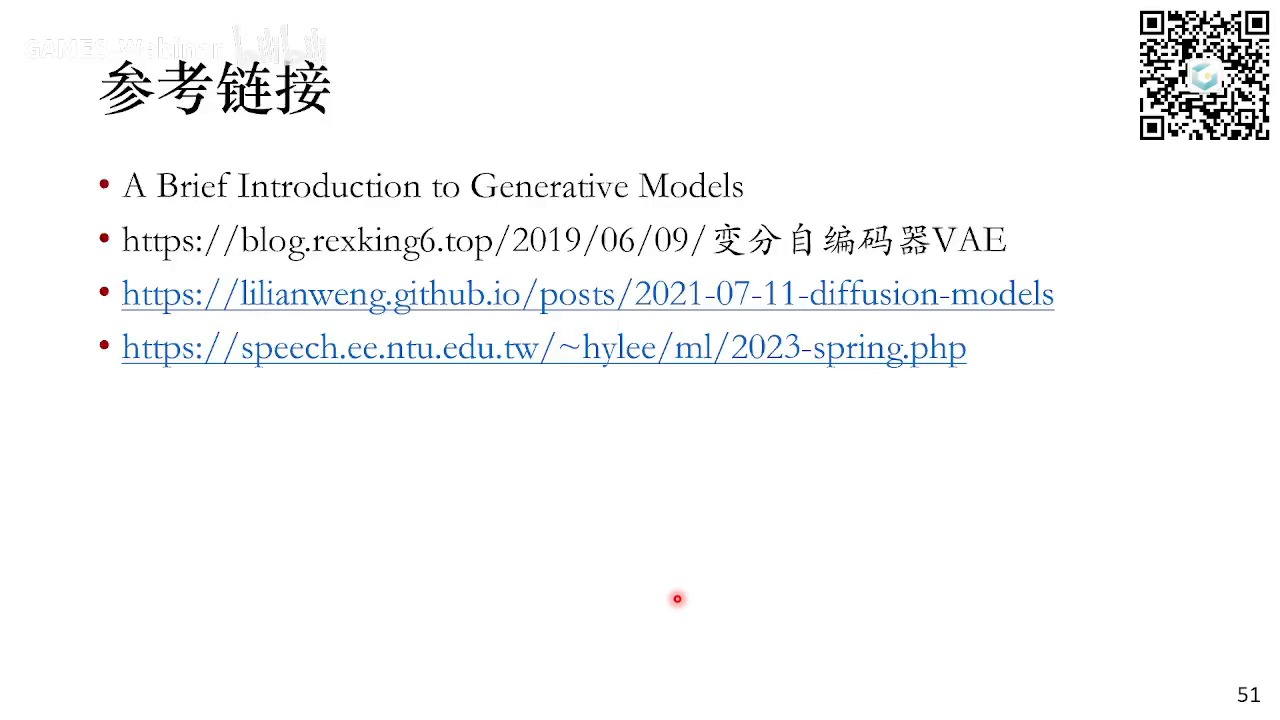
\includegraphics[width=0.92\textwidth]{figures/fig_43_references.jpg}
\caption{参考链接\vtag}
\end{figure}
\srcnote{01:19:45--01:20:00}
\end{minipage}


讲者给出的参考资料包括：《A Brief Introduction to Generative Models》、一篇关于变分自编码器的中文博客、Lilian Weng 关于扩散模型的博客文章，以及台湾大学李宏毅老师 2023 年春季的机器学习课程。

\begin{practicebox}{自测}
\begin{enumerate}
\item 说明为什么最小化 $\mathrm{KL}(p_{\text{data}}\|\pi_\theta)$ 等价于最大似然估计，而最小化 $\mathrm{KL}(\pi_\theta\|p_{\text{data}})$ 则不是。
\item 写出 VAE 损失函数的两项，并解释去掉 KL 项后会发生什么。
\item 由 $x_t=\sqrt{\alpha_t}x_{t-1}+\sqrt{1-\alpha_t}\varepsilon$ 推出 $x_t=\sqrt{\bar\alpha_t}x_0+\sqrt{1-\bar\alpha_t}\varepsilon_t$，用到了哪个定理？
\item 说明为什么扩散模型训练时每张图片只需随机采样一个时刻 $t$，而不需要跑完整个前向过程。
\end{enumerate}
\end{practicebox}

\end{document}
